%Version 3.1 December 2024
% See section 11 of the User Manual for version history
%
%%%%%%%%%%%%%%%%%%%%%%%%%%%%%%%%%%%%%%%%%%%%%%%%%%%%%%%%%%%%%%%%%%%%%%
%%                                                                 %%
%% Please do not use \input{...} to include other tex files.       %%
%% Submit your LaTeX manuscript as one .tex document.              %%
%%                                                                 %%
%% All additional figures and files should be attached             %%
%% separately and not embedded in the \TeX\ document itself.       %%
%%                                                                 %%
%%%%%%%%%%%%%%%%%%%%%%%%%%%%%%%%%%%%%%%%%%%%%%%%%%%%%%%%%%%%%%%%%%%%%

%%\documentclass[referee,sn-basic]{sn-jnl}% referee option is meant for double line spacing

%%=======================================================%%
%% to print line numbers in the margin use lineno option %%
%%=======================================================%%

%%\documentclass[lineno,pdflatex,sn-basic]{sn-jnl}% Basic Springer Nature Reference Style/Chemistry Reference Style

%%=========================================================================================%%
%% the documentclass is set to pdflatex as default. You can delete it if not appropriate.  %%
%%=========================================================================================%%

%%\documentclass[sn-basic]{sn-jnl}% Basic Springer Nature Reference Style/Chemistry Reference Style

%%Note: the following reference styles support Namedate and Numbered referencing. By default the style follows the most common style. To switch between the options you can add or remove �Numbered� in the optional parenthesis. 
%%The option is available for: sn-basic.bst, sn-chicago.bst%  
 
%%\documentclass[pdflatex,sn-nature]{sn-jnl}% Style for submissions to Nature Portfolio journals
%%\documentclass[pdflatex,sn-basic]{sn-jnl}% Basic Springer Nature Reference Style/Chemistry Reference Style
\documentclass[pdflatex,sn-mathphys-num]{sn-jnl}% Math and Physical Sciences Numbered Reference Style
%%\documentclass[pdflatex,sn-mathphys-ay]{sn-jnl}% Math and Physical Sciences Author Year Reference Style
%%\documentclass[pdflatex,sn-aps]{sn-jnl}% American Physical Society (APS) Reference Style
%%\documentclass[pdflatex,sn-vancouver-num]{sn-jnl}% Vancouver Numbered Reference Style
%%\documentclass[pdflatex,sn-vancouver-ay]{sn-jnl}% Vancouver Author Year Reference Style
%%\documentclass[pdflatex,sn-apa]{sn-jnl}% APA Reference Style
%%\documentclass[pdflatex,sn-chicago]{sn-jnl}% Chicago-based Humanities Reference Style

%%%% Standard Packages
%%<additional latex packages if required can be included here>

\usepackage{graphicx}%
\usepackage{multirow}%
\usepackage{amsmath,amssymb,amsfonts}%
\usepackage{amsthm}%
\usepackage{mathrsfs}%
\usepackage[title]{appendix}%
\usepackage{xcolor}%
\usepackage{textcomp}%
\usepackage{manyfoot}%
\usepackage{booktabs}%
%% \usepackage{algorithm}%
%% \usepackage{algorithmicx}%
%% \usepackage{algpseudocode}%
\usepackage{listings}%
%%%%

%%%%%=============================================================================%%%%
%%%%  Remarks: This template is provided to aid authors with the preparation
%%%%  of original research articles intended for submission to journals published 
%%%%  by Springer Nature. The guidance has been prepared in partnership with 
%%%%  production teams to conform to Springer Nature technical requirements. 
%%%%  Editorial and presentation requirements differ among journal portfolios and 
%%%%  research disciplines. You may find sections in this template are irrelevant 
%%%%  to your work and are empowered to omit any such section if allowed by the 
%%%%  journal you intend to submit to. The submission guidelines and policies 
%%%%  of the journal take precedence. A detailed User Manual is available in the 
%%%%  template package for technical guidance.
%%%%%=============================================================================%%%%

%% as per the requirement new theorem styles can be included as shown below
\theoremstyle{thmstyleone}%
\newtheorem{theorem}{Theorem}%  meant for continuous numbers
%%\newtheorem{theorem}{Theorem}[section]% meant for sectionwise numbers
%% optional argument [theorem] produces theorem numbering sequence instead of independent numbers for Proposition
\newtheorem{proposition}[theorem]{Proposition}% 
%%\newtheorem{proposition}{Proposition}% to get separate numbers for theorem and proposition etc.
%% private
%% %% \newtheoremrep{definition}{Definition}[section]
%% \newtheoremrep{lemma}[theorem]{Lemma}[section]
%% \newtheoremrep{proposition}[proposition]{Proposition}[section]
%% %% \newtheoremrep{theorem}[theorem]{Theorem}[section]
%% \newtheoremrep{corollary}[theorem]{Corollary}[section]
%% %% \newtheoremrep{remark}[theorem]{Remark}

\theoremstyle{thmstyletwo}%
\newtheorem{example}{Example}%
\newtheorem{remark}{Remark}%
\theoremstyle{thmstylethree}%
\newtheorem{definition}{Definition}%
%% send a proof to the appendix

\raggedbottom
%%\unnumbered% uncomment this for unnumbered level heads

%%%%%%%%%%%%%%%%%%%%%%%%%%%%%%%%%%%%%%%
%%% private macros
\usepackage{graphicx}
\usepackage[appendix=strip]{apxproof}%default
\graphicspath{
  {fig/}
  {fig/exp1/}
  {fig/fig1/}
  {fig/turu/}
}%%
%%% config.tex

%%======================================
\usepackage{graphicx}
%% \usepackage{amsmath,amssymb}
%% \usepackage{mathtools}
%% \mathtoolsset{showonlyrefs=false} %% 参照している式参照のみ表示
%% \mathtoolsset{showonlyrefs=true} %% 参照している式参照のみ表示
%% \usepackage{cite}
\usepackage{caption}    %%for subfigure
\usepackage[skip=0.5ex]{subcaption} %%for subfigure
\captionsetup{aboveskip=0.0\baselineskip}
\captionsetup{belowskip=0.0\baselineskip}
%%%
%%\usepackage{titlesec}
%% \titlespacing*{\section}{0pt}{5.5ex plus 1ex minus .2ex}{4.3ex plus .2ex}
%% \titlespacing*{\subsection}{0pt}{5.5ex plus 1ex minus .2ex}{4.3ex plus .2ex}

%%% table
%% \usepackage{multirow}
\usepackage{booktabs}
\usepackage{array}

% private macros by others 
\usepackage{url}
\usepackage{bm}
\usepackage{textcomp}%%for cent
%\usepackage[margin=1.75in]{geometry}
%\usepackage[margin=1.0in]{geometry}
%% \usepackage{subfig}
%% \usepackage{natbib}

%%% private %%%%%%%%%%%%%%%%%%%%%%%%%%%%%%%%%%%%%

%% private macros by arim@ist
%%% jsvmac.tex
%%% macros from a subset of jsv1.sty 

%%% from jsv1.sty

% Write multichar identifier names using \id in either mathmode or text;
% For ex, $\id{high}(x)$ is an expression using the \id{high} function.
% Use ``\ '' if a space is desired, as in math mode.
\def\id#1{\ensuremath{\mathit{#1}}}
\let\idit=\id
\def\idbf#1{\ensuremath{\mathbf{#1}}}
\def\idrm#1{\ensuremath{\mathrm{#1}}}
\def\idtt#1{\ensuremath{\mathtt{#1}}}
\def\idsf#1{\ensuremath{\mathsf{#1}}}
\def\idcal#1{\ensuremath{\mathcal{#1}}}  % Use with capital letter args only
\def\idsc#1{\ensuremath{\textsc{#1}}} % added by arim

%%% end jsv1.sty

%%% EOF

%%\input{arimmacro} %%privatemacro


%%%%%%%%%%%%%%%%%%%%%%%%%%%%%%%%%%%%%%%%
%%xsavebox
\usepackage{xsavebox}

%%%%%%%%%%%%%%%%%%%%%%%%%%%%%%%%%%%%%%%%%
%%% above and below float figure table
\setlength\intextsep{0.5\baselineskip}
\setlength\abovecaptionskip{0.0\baselineskip}
\setlength\belowcaptionskip{0.5\baselineskip}
%% \setlength\intextsep{18pt}

%%%%%%%%%%%%%%%%%%
%% latex native savebox and lrbox
\newenvironment{savethm}[1]{\begin{lrbox}{#1}\begin{minipage}[t]{1.0\textwidth}}{\end{minipage}\end{lrbox}}

\newcommand{\putthm}[1]{
%% \smallskip
\noindent 
\usebox{#1}
\medskip}

%%sample
%% \newsavebox{\thmbox}
%% \begin{lrbox}{\thmbox}
%% \begin{minipage}[t]{1.0\textwidth}
%% \begin{theorem}\label{thm:algbwt:main}
%% ....
%% \end{theorem}
%% \end{minipage}
%% \end{lrbox}


%% \putthm{\thmbox}


%%%%%%%%%%%%%%%%%%




%%%%%%%%%%%%%%%%%%%%%%%%%%%%%%%%%%%%%%%%
%%comment out a paragraph
\newsavebox{\cmbox}
\newenvironment{commbox}{
  \begin{lrbox}{\cmbox}
    \begin{minipage}{.9\textwidth}
}{\end{minipage}
  \end{lrbox}
  %\framebox{\usebox{\cmbox}}
}


%%%%%%%%%%%%%%%%%%%%%%%%%%%%%%%%%%%%%%%%
% %%% empty environment 
% \newenvironment{myempty}{\begin{commbox}}{\end{commbox}}
% %%% proof environment 
% \newenvironment{myproof}{\begin{proof}}{\end{proof}} %default
% \newenvironment{myfullproof}{\begin{proof}}{\end{proof}} %default
% \newenvironment{myfullproofempty}{\begin{myempty}}{\end{myempty}} %default

%% replace an enviroment #1 with #2
\newcommand{\myenvironmentreplace}[2]{\renewenvironment{#1}{\begin{#2}}{\end{#2}}}

%% claim %%
\newenvironment{myclaim}[1][]{\bgroup\parskip=0mm\par (\textit{Claim{#1}})}{(\textit{End of Claim})\par\egroup}  
\newenvironment{proofofclaim}{\bgroup\parindent=1em\parskip=0mm\par (\textit{Proof for the claim})}{(\textit{End of the proof for the claim})\par\egroup}  
\newenvironment{proofofclaimempty}{\begin{myempty}}{\end{myempty}}

%% \newenvironment{proofofclaim}{\bgroup\parskip=0mm\par (Proof for the claim)}{(End of the proof for the claim)\par\egroup}  


%%%%%%%%%%%%%%%%%%%%%%%%%%%%%%%%%%%%%%%%

% %% switch catcode of '&' between 4 and 9
% \newenvironment{inalign}{\begin{math}\catcode`&=9}{\catcode`&=4\end{math}}

%%%%%%%%%%%%%%%%%%%%%%%%%%%%%%%%%%%%%%%%

% lipics predefined

%% send a proof to the appendix
\newtheorem{definition}{Definition}
\newtheorem{theorem}{Theorem}
\newtheorem{lemma}[theorem]{Lemma}
\newtheorem{proposition}{Proposition}
\newtheorem{corollary}[theorem]{Corollary}
\newtheorem{remark}{Remark}
\newtheorem{fact}{Fact}
\newtheorem{condition}{Condition}

% \newtheorem{example}[example]{Example}[section]
% \newtheorem{conjecture}{Conjecture}
% %% dammy
%%%%%%%%%%%%%%%%%%%%%%%%%%%%%%%%%%%%%%%%

%%% cleveref
\usepackage{cleveref}
\crefname{section}{Sec.}{Sections}
\crefname{chapter}{Chapter}{Chapters}
%%
\crefname{algorithm}{Algorithm}{Algorithms}
\crefname{table}{Table}{Tables}
\crefname{figure}{Fig.}{Figures}
%% 
\crefname{definition}{Definition}{Definitions}
\crefname{lemma}{Lemma}{Lemmas}
\crefname{proposition}{Prop.}{Propositions}
\crefname{theorem}{Theorem}{Theorems}
\crefname{remark}{Remark}{Remarks}
\crefname{fact}{Fact}{Facts}
\crefname{condition}{Condition}{Conditions}
\crefname{problem}{Problem}{Problems}
\crefname{observation}{Observation}{Observations}
%% \crefname{lemma}{Lemma}{Lemmas}
\crefname{equation}{Eq.}{Equations}
%%% fix of a bug in Algorithm
\newcommand{\aref}[1]{Algorithm\kern0.25em\ref{#1}} 
%%%%%%

% %% send a proof to the appendix
\usepackage{apxproof}
% \newtheoremrep{definition}{Definition}[section]
\newtheoremrep{lemma}[theorem]{Lemma}[section]
\newtheoremrep{proposition}[proposition]{Proposition}[section]
\newtheoremrep{theorem}[theorem]{Theorem}[section]
\newtheoremrep{corollary}[theorem]{Corollary}[section]
% \newtheoremrep{remark}[theorem]{Remark}

%% \newtheoremrep{example}[example]{Example}[section]
%% \newtheoremrep{conjecture}{Conjecture}
%% %% dammy
%% \newcommand{\resetrep}{}
%% rest 
%% \newcommand{\resetreptext}{{\rm\textsf{in draft}}}
%% \newcommand{\getfollow}[1][{}]{{\rm\textsf{(*{#1})}}\ }

%% \newcommand{\resetrep}{%% resetting all rep-style environments
%% %% \renewenvironment{lemmarep}{\begin{lemma}\getfollow}{\end{lemma}}
%% \renewenvironment{lemmarep}{\begin{lemma}\getfollow}{\end{lemma}}
%% \renewenvironment{propositionrep}{\begin{proposition}\getfollow}{\end{proposition}}
%% \renewenvironment{theorem}{\begin{theorem}\getfollow}{\end{theorem}}
%% \renewenvironment{corollaryrep}{\begin{corollary}\getfollow}{\end{corollary}}
%% \renewenvironment{examplerep}{\begin{example}\getfollow}{\end{example}}
%% \renewenvironment{remarkrep}{\begin{remark}\getfollow}{\end{remark}}
%% \renewenvironment{conjecturerep}{\begin{conjecture}\getfollow}{\end{conjecture}}
%% \renewenvironment{toappendix}{}{}
%% }

%%%%% 
\newenvironment{statement}[1]{\begin{trivlist}\item[]$\blacktriangleright\:$\textbf{#1}\ }{\end{trivlist}}
\newenvironment{notoappendix}{}{} %% the empty version of toappendix

%%%%%%%%%%%%%%%%%%%%%%%%%%%%%%%%%%%%%%%%%
%% enumitem: smart enumerate and itemize
%% the vspace above list = \topsep + \parskip + \partopsep
%% the vspace between items = \itemsep + \Parsep 
%% the vspace between paragraphs = \Parsep 
\usepackage[inline,shortlabels]{enumitem} %enumerate
\setlist{noitemsep}
\setlist{%
topsep = 0.25\baselineskip,
parsep = 0.125\baselineskip
}%exp
\setlist[enumerate]{ labelsep=.25pc, leftmargin=1.5pc } 
%% \setlist[enumerate]{ labelsep=.25pc, leftmargin=1.5pc } 
\setlist[enumerate,1]{ label= (\arabic*), ref=\arabic*}
\setlist[enumerate,2]{ label= (\roman*),ref  = \roman*}
\setlist[enumerate,3]{ label= (\alph*), ref  = (\alph*)}
%\setlist[itemize]{ leftmargin=1.5pc }
\setlist[description]{ font=\sffamily\bfseries }
%% end macros
%%% switch
%% \newenvironment{myenumerate}{\begin{enumerate}}{\end{enumerate}}
\newenvironment{myenumerate}{\begin{enumerate*}}{\end{enumerate*}}
%% end macros

%%

%% %% 目次のハイパーリンク: 印刷時は念の為コメントアウト(本来出ない)
%% \usepackage[%
%% %dvipdfmx,%
%% colorlinks=true,%
%% linkcolor=blue,%
%% anchorcolor=black,%
%% citecolor=blue,%
%% urlcolor=blue%
%% ]{hyperref} %注意:パッケージの最後に読み込むこと

%%%%

%% EOF

% macros.tex

%%%%%%%%%%%%%%%%%%%%%%%%%%%%%%%%%%%%%%%%%
%% reference with [] in environment 
\def\refbox(#1){$\mbox{\bf ({#1}) }$}
\newcommand{\mysubsubsection}[1]{\textbf{#1}.\hspace{0.125em}}%% camera
%% \newcommand{\mysubsection}[1]{\subsection*{#1}}

%% private macros: cdawg
%% class names
\newcommand{\suffix}{\id{Suffix}}
\newcommand{\substr}{\id{Substr}}
\newcommand{\prefix}{\id{Prefix}}
\newcommand{\Suf}{\suffix}
\newcommand{\Substr}{\substr}
\newcommand{\Pref}{\prefix}
%%% 
\newcommand{\lext}[1]{\overleftarrow{#1}} 
\newcommand{\rext}[1]{\overrightarrow{#1}} 
\newcommand{\mext}[1]{\overleftrightarrow{#1}}
\newcommand{\str}{\op{str}}
%%%
\newcommand{\spos}[1][S]{\op{Spos}_{#1}}
\newcommand{\epos}[1][S]{\op{Epos}_{#1}}
\newcommand{\occ}[1][]{\op{Occ}_{#1}}
%% maximal 
\newcommand{\RM}{\sig{RM}}
\newcommand{\LM}{\sig{LM}}
\newcommand{\M}{\sig{M}}
%%%%
\newcommand{\rstate}[1]{[{#1}]_{\equiv_R}}
\newcommand{\lstate}[1]{[{#1}]_{\equiv_L}}
%%%
\newcommand{\BUSA}{\textsf{BUSA}} 
\newcommand{\TDSA}{\textsf{TDSA}} 
\newcommand{\TDBW}{\textsf{TDBW}}
%%%
\newcommand{\MAW}{\idit{MAW}} 
\newcommand{\MUS}{\idit{MUS}} 
\newcommand{\MRW}{\idit{MRW}} 
\newcommand{\MRWK}[1][k]{\mbox{$#1$-\idit{MRW}}}
%%%%
%%% data structures
\newcommand{\stree}{\id{STree}}%exp
\newcommand{\weiner}{\id{Weiner}}%exp
\newcommand{\CDAWG}{\mathit{CDAWG}}
\newcommand{\SA}{\id{SA}}
\newcommand{\ISA}{\id{ISA}}
\newcommand{\BWT}{\id{BWT}}
\newcommand{\LCP}{\id{LCP}}
\newcommand{\LCE}[1][T]{\idrm{LCE}_{#1}}
%%%
\newcommand{\repr}{\op{repr}}
\newcommand{\intr}{\op{SA\textrm{-}Int}}
\newcommand{\lcpmin}{\op{lcpmin}}
%%%%
\newcommand{\set}[1]{\{\kern0.05em#1\kern0.05em\}}
\newcommand{\sete}[1]{\{\kern0.2em#1\kern0.2em\}}
\newcommand{\liste}[1]{[\kern0.2em#1\kern0.2em]}

%%%%
%\newcommand{\mywspace}[1][R]{O(\sigma^2\log e_{#1})}
%% \newcommand{\td}{\idsf{Td}}
%% \newcommand{\bu}{\idsf{Bu}}
%% \newcommand{\fw}{\idsf{Fwd}}
%% \newcommand{\bw}{\idsf{Bwd}}
\newcommand{\td}{\idsf{T}}
\newcommand{\bu}{\idsf{B}}
\newcommand{\fw}{\idsf{F}}
\newcommand{\bw}{\idsf{B}}
\newcommand{\tdfw}{\mbox{\td\fw}}
\newcommand{\tdbw}{\mbox{\td\bw}}
\newcommand{\bufw}{\mbox{\bu\fw}}
\newcommand{\bubw}{\mbox{\bu\bw}}
\newcommand{\tdfwd}{\tdfw}%% obsolute 
\newcommand{\tdbwd}{\tdbw}%% obsolute 
\newcommand{\bufwd}{\bufw}%% obsolute 
\newcommand{\bubwd}{\bubw}%% obsolute 
% %%% 

%%%%%%%%%%%%%%%%%%%%%%%%%%%%%%%%%%%%%%%%%
\usepackage{yhmath}%% for neat wide tilde

%%%%%%%%%%%%%%%%%%%%%%%%%%%%%%%%%%%%%%%%%

%% basis 
\renewcommand{\-}{\mbox{\textit{-}}}

%% symbols
\newcommand{\nat}{\mathbb{N}}
\newcommand{\rat}{\mathbb{R}}
\newcommand{\zat}{\mathbb{Z}}
\renewcommand{\leq}{\leqslant}%override
\renewcommand{\le}{\leqslant}%override
\renewcommand{\preceq}{\preccurlyeq}%override
\newcommand{\rev}{^\fn{rev}}

%% typeface 
\newcommand{\proc}[1]{\mbox{\textsf{#1}}}
\newcommand{\algo}[1]{\mbox{\textsf{#1}}}
\newcommand{\fn}[1]{\ensuremath{\mathrm{#1}}} 
\newcommand{\mb}[1]{\mathbb{#1}}
\newcommand{\name}[1]{\textit{#1}}

\newcommand{\eps}{\varepsilon}
\newcommand{\daller}{\$} %$
\renewcommand{\sharp}{\#} %$
\newcommand{\mathdaller}{\mbox{`$\daller$'}} %$
\newcommand{\centsymbol}{\mbox{\textcentoldstyle}} %$
\DeclareMathOperator{\polylog}{\mathrm{polylog}}

\newcommand{\kw}[1]{\textbf{#1}}
\newcommand{\sig}[1]{\mathcal{#1}}
\newcommand{\ty}[1]{\texttt{#1}}
%% \newcommand{\op}[1]{\mathtt{#1}}
%% \renewcommand{\-}{\mbox{-}}
\newcommand{\mop}[1]{\mbox{\rm\texttt{#1}}}%%exp
\newcommand{\op}[1]{\mathtt{#1}}


%% math: general 
\newcommand{\by}{\times}
\renewcommand{\bar}[1]{\overline{#1}}
\newcommand{\ceil}[1]{\lceil #1\rceil}
\newcommand{\floor}[1]{\lfloor #1\rfloor}
%\newcommand{\Implies}{\:\:}
\renewcommand{\iff}{\mathbin{\,\Leftrightarrow\,}}%override
\newcommand{\iffdef}{\mathbin{\,\stackrel{\textrm{def}}{\iff}\,}}
\newcommand{\Implies}{\mathbin{\,\Rightarrow\,}}%override
\newcommand{\To}{\Implies}%override
%% \newcommand{\iffshort}{\Leftrightarrow} %%short
\newcommand{\indicator}[1]{\mathbb{I}\kern-0.1em\left[\kern0.1em{#1}\kern0.1em\right]}
\newcommand{\pair}[1]{\langle #1\rangle}
%% \renewcommand{\mid}{\,:\,}
\newcommand{\infrac}[2]{{#1}\,/\,{#2}} %inline frac

%% not used 
\newcommand{\pow}[1]{2^{#1}}
\newcommand{\rng}[3]{_{#1=#2}^{#3}}
%% \renewcommand{\vec}[1]{\mathbf{#1}}
\newcommand{\rk}[1]{^{(#1)}}
\newcommand{\rkk}[1]{^{\kern.5pt\textrm{#1}}}


%%% tentative
\DeclareMathOperator{\pd}{..}
%%% tex hack: ".."コマンドを作成する
%%% https://tex.stackexchange.com/questions/4216/how-to-typeset-correctly
% \mathchardef\ordinarycolon\mathcode`\.
%%% raise: http://www.math.kobe-u.ac.jp/HOME/kodama/tips-latex-math-margin.html#raise 
\mathcode`\.=\string"8000
\begingroup \catcode`\.=\active
  \gdef.{\hbox{\hskip1pt\raise-2pt\hbox{$\cdot$\hskip1pt}}}
\endgroup
%%% end tex hack


%%% setting: algorithm2e %%%%%%%%%%%%%%%%%%%%%%%%%%%%%%%%
\newcommand{\algoopts}{%
%%% RULES
%boxed,%good
%boxruled,%
%algoruled,%good
ruled,%
%tworuled,%
%%% CODE TYPESETTING
%% hangingcomment,%
%% opthanginginout,%
%% noalgohanging,%obsolute 
%%% BLOCKS DISPLAY
%noline,%
vlined,%L-tyle
%lined,%I-style
%%%
linesnumbered%
}
%%\usepackage[\algoopts]{algorithm2e} 
\usepackage[ruled,vlined,linesnumbered]{algorithm2e} 

\makeatletter
\renewcommand{\@algocf@capt@plain}{above}% formerly {bottom}
\makeatother
%%% algorithm2e
\newcommand{\Commentblock}[1]{\hfill$\rhd$\ \textit{#1}}
\newcommand{\Commentblockl}[1]{\kern0.5em$\rhd$\ \textit{#1}\ $\lhd$}
\newcommand{\CM}[1]{\Commentblock{#1}}
%% \SetArgSty{textrm}%arguments for e.g., if, else, while etc. 
%% \SetCommentSty{textit}%arguments for comments
\SetKwComment{Comment}{$\rhd$}{} 
\SetKwInput{KwGiven}{Given}
\SetKwInput{KwGlobal}{Global}
\SetKwInput{KwWork}{Working}
\SetArgSty{textrm}%arguments for e.g., if, else, while etc. 
\SetCommentSty{textit}%arguments for comments
\newcommand{\iIf}[2]{\textbf{if} {#1} \textbf{then}\hspace{0.125em}{\relax #2}}
\newcommand{\iElseIf}[2]{\textbf{else if} {#1} \textbf{then}\hspace{0.125em}{\relax #2}}
\newcommand{\iElse}[1]{\textbf{else} {\relax #1}}

%%%%%%%%%%%%%%%%%%%%%%%%%%%%%%%%%%%%%%%%%%%%%%%%%%%%%%%%%
%%
%%% 
%% \newcommand{\up}{--}
\newcommand{\up}{{\mbox{--}}}
\newcommand{\dw}{+}
\newcommand{\down}{\dw}%% for compatibility 
%% \newcommand{\up}{\idrm{up}}
%% \newcommand{\down}{\idrm{dw}}

%% private macros: cdawg
\newcommand{\inv}{^{-1}}
\newcommand{\anc}{\idrm{anc}}
\newcommand{\lex}{\idrm{lex}}
\newcommand{\len}{\idrm{len}}
\newcommand{\pos}{\idrm{pos}}
\newcommand{\no}{\idrm{no}}
\newcommand{\idx}{\op{idx}}
\newcommand{\val}{\op{val}}
%%
\newcommand{\Path}[1][(G)]{\idtt{Path}{#1}}%exp

%%% 
\renewcommand{\S}{\mathcal{S}} 
%%\renewcommand{\S}{\mathcal{U}} 
\newcommand{\U}[1][\delta]{\mathcal{U}_{#1}} 
\newcommand{\PS}[1][\delta]{\idtt{Path}_{#1}} 
\newcommand{\R}{\mathcal{D}}
\renewcommand{\SS}[1][\le_\pos]{\S^{#1}} %% orig:\S := 'section'
\newcommand{\RR}[1][\preceq]{\R^{#1}}
%%% an edge 
\newcommand{\lab}{\op{lab}}
\newcommand{\src}{\op{src}}%%tail
\newcommand{\dst}{\op{dst}}%%head
\newcommand{\tail}{\src}%%tail
\newcommand{\head}{\dst}%%head
\newcommand{\tl}{\tail}%%tail
\newcommand{\hd}{\head}%%head
%%% 
\newcommand{\fstchar}{\mop{fstchar}}
\newcommand{\elen}{\mop{len-edge}}
%%% canonical suffix 
\newcommand{\cano}[1][\delta]{\op{cano}_{#1}}
%% \newcommand{\cano}{\op{cano}}
\newcommand{\spath}[1][]{\op{SP}_{#1}}
%% \newcommand{\spath}{\op{SP}}
\newcommand{\precsym}{\op{precsym}}
%%%%%%%%%%%%%%%%%%%%%%%%%%%%%%%%%
\newcommand{\Pos}{\op{pos}}
\newcommand{\Rnk}{\op{rnk}}
%%%%%%%%%%%%%%%%%%%%%%%%%%%%%%%%%%
%%%%%% canonical suffix 
\newcommand{\COBJ}[3]{\mathrm{#1}_{#3}(T, {\lequp}, {#2})}
\newcommand{\CS}[1][\delta]{\sig{CS}_{#1}(G)}
\newcommand{\SP}[1][\delta]{\sig{SP}_{#1}(G)}
\newcommand{\CE}[1][\delta]{\sig{CE}_{#1}}
%% \newcommand{\Cert}[1][\delta]{\mathrm{Cert}_{#1}(T)}
%% \newcommand{\CE}{\sig{CE}}
\newcommand{\RSA}{\mathsf{SA}}%%
\newcommand{\comp}[1]{\overline{#1}}%%
%%
\newcommand{\vobj}[2][\delta]{\bm{#2}_{#1}}%virtual object
\newcommand{\trivcsuf}[1][\delta]{\vobj[#1]{S}}
\newcommand{\trivsuf}[1][\delta]{\vobj[#1]{S}}
\newcommand{\trivedge}[1][\delta]{\vobj[#1]{f}}
\newcommand{\trivnode}[1][\delta]{\vobj[#1]{\bot}}
%%%%%% 
\newcommand{\SPath}[1][\lequp]{\mathit{SPath}(G,{#1})}
\newcommand{\RSPath}[1][\leqdw]{\mathit{RSPath}(G,{#1})}
%% \newcommand{\CS}{\CSuf}%obsolute
\newcommand{\csuf}{\op{csuf}}%
\newcommand{\csufup}{\op{csuf}_{\up}}%
\newcommand{\csufdw}{\op{csuf}_{\dw}}%
\newcommand{\cspath}{\op{cspath}}%obsolute
%%%
\newcommand{\dom}{\op{dom}}%exp
\newcommand{\codom}{\op{co\-dom}}%exp
%%%
\newcommand{\BIrrPos}{\idrm{IrrPos}(T)}
\newcommand{\BIrrRnk}{\idrm{IrrRnk}(T)}
\newcommand{\QIrrPos}[1][\leqdw]{\idrm{QIrrPos}(T, {#1})}
\newcommand{\QIrrRnk}[1][\leqdw]{\idrm{QIrrRnk}(T, {#1})}
\newcommand{\BIrr}{BIrrXXX}
\newcommand{\QIrr}{QIrrXXX}
\newcommand{\Irr}{IrrXXX}
%%% 
\newcommand{\interp}{\op{interpolate}}
\newcommand{\Parse}{\op{parse}}%lncs3
%% up and down
%% terminals
%% \renewcommand{\up}{\idrm{up}}
%% \renewcommand{\dw}{\idrm{dw}}
%% path ordering 
\newcommand{\less}{<}%%for compatibility
\newcommand{\leqp}[1][\delta]{\mathbin{\preceq_{#1}}}
\newcommand{\lessp}[1][\delta]{\mathbin{\prec_{#1}}}
\DeclareMathOperator{\lequp}{\mbox{$\leqp[\up]$}}
\DeclareMathOperator{\lessup}{\mbox{$\lessp[\up]$}}
\DeclareMathOperator{\leqdw}{\mbox{$\leqp[\down]$}}
\DeclareMathOperator{\lessdw}{\mbox{$\lessp[\down]$}}
\DeclareMathOperator{\leqdown}{\leqdw}
%%% pos and lex 
\DeclareMathOperator{\leqpos}{\leqp[\pos]}
\DeclareMathOperator{\lesspos}{\lessp[\pos]}
\DeclareMathOperator{\leqlex}{\leqp[\lex]}
\DeclareMathOperator{\lesslex}{\lessp[\lex]}
%%% edge order 
\newcommand{\leqedge}{\leq^E}
\newcommand{\lessedge}{<^E}
%% \DeclareMathOperator{\lessedge}{<^E}
\newcommand{\leqe}[1][\delta]{{\leqedge_{#1}}}
\newcommand{\leqein}{\leqe[-]}
\newcommand{\leqeout}{\leqe[+]}
\newcommand{\lesse}[1][\delta]{{\lessedge_{#1}}}
\newcommand{\lessein}{{\lesse_{-}}}
\newcommand{\lesseout}{{\lesse_{+}}}
%%% edge 
\newcommand{\leqa}[1][\delta]{{\leqedge_{#1}}}
\newcommand{\leqepos}[1][-]{\leq^{E}_{#1,\pos}}%up:dw \leqepos[-]
\newcommand{\leqelex}[1][+]{\leq^{E}_{#1,\lex}}%dw only \leqelex[+]
\newcommand{\lessepos}[1][-]{<^{E}_{#1,\pos}}%up:dw \lessepos[-]
\newcommand{\lesselex}[1][+]{<^{E}_{#1,\lex}}%dw only \lesselex[+]
%%%
\DeclareMathOperator{\leqeoutlex}{{\leq^E_{+,\lex}}}
\DeclareMathOperator{\lesseoutlex}{{<^E_{+,\lex}}}
\DeclareMathOperator{\leqeinpos}{{\leq^E_{--,\pos}}}
\DeclareMathOperator{\lesseinpos}{{<^E_{--,\pos}}}
%% total orders 
\newcommand{\isprimary}[1][\delta]{\mop{is-primary}_{#1}}
\newcommand{\shortest}[1][\delta]{\mop{shortest}_{#1}}
%%% representative: 
\newcommand{\nleaves}{\mop{nleaves}}%\#\U[+]
\newcommand{\leftmostrank}{\mop{leftmost-rank}}%
%%% spanning tree
\newcommand{\TU}{\sig{T}_\up} %%forward tree = donward spanning tree
\newcommand{\TD}{\sig{T}_\dw} %%reverse tree = upward spanning tree
%%%%%%

\newcommand{\mypreceq}{{\leqdw}}%exp
\newcommand{\myprec}{{\lessdw}}%exp
\newcommand{\qir}[1]{{\widetilde{#1}}}
\newcommand{\bir}[1]{{\widehat{#1}}}
\newcommand{\GLPF}{\idit{GLPF}}
\newcommand{\GLPFd}{\GLPF_{\scriptsize\mypreceq}}%exp
\newcommand{\GLPFdq}[1][\leqdw]{\qir{\idit{GLPF}}_{\scriptsize #1}}
\newcommand{\GLPnF}{GLPnF}
\newcommand{\IPOS}[1][\preceq]{\mathcal{IRR}_{#1}}
\newcommand{\F}[1][]{\mathcal{F}_{#1}}
\newcommand{\V}[1][]{\mathcal{V}_{#1}}
\newcommand{\E}[1][]{\mathcal{E}_{#1}}
\renewcommand{\root}{\id{root}}% 
\newcommand{\sink}{\id{sink}}% 
\newcommand{\suf}{\id{suf}}% 
%%% edges and neigbors
\newcommand{\N}[1][\delta]{N_{#1}}
\newcommand{\In}{\N[-]}
\newcommand{\Out}{\N[+]}
%% \newcommand{\In}{N_{-}}
%% \newcommand{\Out}{N_{+}}
%% \newcommand{\In}{\op{In}}
%% \newcommand{\Out}{\op{Out}}
%% \newcommand{\EEE}[2]{\mbox{$\mathcal{E}_{\scriptsize #1}^{\scriptsize #2}$}}
%% \newcommand{\EEE}[3]{\mbox{$\mathcal{#1}_{\scriptsize #3}^{\scriptsize (#2)}$}}
%% \newcommand{\EE}[2]{\mbox{$\mathcal{E}_{\scriptsize #2}^{\scriptsize (#1)}$}}
\newcommand{\EE}[2]{\mbox{$\mathcal{E}_{#2}^{#1}$}}
\newcommand{\EP}[1][\delta]{\EE{\star}{#1}}
\newcommand{\ES}[1][\delta]{\overline{\EE{\star}{#1}}}
\newcommand{\ESX}[1][\delta]{\ES[#1]\cup\set{\trivedge[#1]}}
\newcommand{\T}[1][\delta]{\sig T_{#1}}
%% \newcommand{\EP}[1][\delta]{\EE{1}{#1}}
%% \newcommand{\ES}[1][\delta]{\EE{2}{#1}}
\newcommand{\EPU}[1][]{\EP[\up]}
\newcommand{\ESU}[1][]{\ES[\up]}
\newcommand{\EPD}[1][]{\EP[\dw]}
\newcommand{\ESD}[1][]{\ES[\dw]}
%% \newcommand{\EPU}[1][]{\EE{1{#1}}{\up}}
%% \newcommand{\ESU}[1][]{\EE{2{#1}}{\up}}
%% \newcommand{\EPD}[1][]{\EE{1}{\down #1}}
%% \newcommand{\ESD}[1][]{\EE{2}{\down #1}}
\newcommand{\Emin}{E_{\preceq}^{\min}}


%%%%%%%%%%%%%%%%%%%%%%%%%%%%%%%%%%%%%%%%%%%%%%%%%%%%%%%%%
%%%% helper
\newcommand{\nofbox}[1]{#1}

%% EOF

%for lncs1submit
%%%%%%%%%%%%%%%%%%%%%%%%%%%%%%%%%%%%%%%

\begin{document}

\title[Article Title]{Enumerating Maximal Repeats: Taxonomy and New Algorithm}

%%=============================================================%%
%% GivenName	-> \fnm{Joergen W.}
%% Particle	-> \spfx{van der} -> surname prefix
%% FamilyName	-> \sur{Ploeg}
%% Suffix	-> \sfx{IV}
%% \author*[1,2]{\fnm{Joergen W.} \spfx{van der} \sur{Ploeg} 
%%  \sfx{IV}}\email{iauthor@gmail.com}
%%=============================================================%%

\author*[1,2]{\fnm{Hiroki} \sur{Arimura}}\email{arim@ist.hokudai.ac.jp}

\author[2,3]{\fnm{Shunsuke} \sur{Inenaga}}\email{inenaga.shunsuke.380@m.kyushu-u.ac.jp}
\equalcont{These authors contributed equally to this work.}

\author[1,2]{\fnm{Yuta} \sur{Tsuruzono}}\email{turuzono.yuta.y9@elms.hokudai.ac.jp}
\equalcont{These authors contributed equally to this work.}

\affil*[1]{\orgdiv{Faculty of IST}, \orgname{Hokkaido University}, \orgaddress{\city{Sapporo}, \country{Japan}}}

\affil*[2]{\orgdiv{Graduate School of IST}, \orgname{Hokkaido University}, \orgaddress{\city{Sapporo}, \country{Japan}}}

\affil[3]{\orgdiv{Department of Informatics}, \orgname{Kyushu University}, \orgaddress{\street{Street}, \city{Fukuoka}, \state{State}, \country{Japan}}}
%% \affil*[1]{\orgdiv{Graduate School of IST}, \orgname{Hokkaido University}, \orgaddress{\street{Street}, \city{City}, \postcode{100190}, \state{State}, \country{Japan}}}

%% \affil[2]{\orgdiv{Department}, \orgname{Organization}, \orgaddress{\street{Street}, \city{City}, \postcode{10587}, \state{State}, \country{Country}}}

%% \affil[3]{\orgdiv{Department of Informatics}, \orgname{Kyushu University}, \orgaddress{\street{Street}, \city{Fukuoka}, \postcode{}, \state{State}, \country{Japan}}}

%%==================================%%
%% Sample for unstructured abstract %%
%%==================================%%

\abstract{%%% abst.tex
\begin{abstract}
  This paper addresses the problem of efficiently enumerating unusual words in a string, such as minimal rare words (MRWs). Although existing algorithms are effective, they are not output-dependent, always requiring $\Theta(n)$ time even for a small number of patterns. Our work provides an output-dependent algorithm for enumerating MRWs
  in $O(e_R + e_L + occ)$ time and $O(e_L  + \sigma^2 \log n)$ working space, where $occ$ is the number of distinct patterns, and $e_L$ and $e_R$ are parameters, called the numbers of left- and right-extensions of maximal repeats in S, respectively, which are sublinear for repetitive strings. We introduce a new algorithm to enumerate maximal repeats using a suffix array, LCP array, and BWT array, which is the key to our sublinear time complexity. This is the first result to achieve a sublinear time complexity for this problem.
\end{abstract}

%% denote the numbers of left- and right-extensions of maximal repeats in S, respectively, and are upper-bounded by the length n of the string, and can be sublinear in n, up to logarithmic, for highly repetitive strings such as a collection of human genomes.


%%   In this paper, we study efficient enumeration of classes of unusual words in a string.
%%   %% In this paper, we study efficient enumeration of non-trivial MAWs and other classes of unusual words, such as the \textit{minimal unique substrings} (MUSs) and the \textit{minimal rare words} (MRWs) in a string.
%%   A \textit{minimal absent word} (MAW) of a string $S$ is a string $w$ that does not occur in $S$ and any proper substring of $w$ occurs in $S$ as a substring. For any integer $k\ge 0$, as most general form of unusual word, a \textit{minimal rare word} (MRW) of $S$ with frequency $k$ is any string $w$ that occurs in $S$ exactly $k$ times, and any proper substring of $w$ has strictly less occurrences in $S$. An unusual word is said to be non-trivial if it has length at least two.
%% Presently, most practical algorithms for unusual words use the suffix array or the Burrows-Wheeler transform of $S$ rather than space inefficient data structures such as the suffix trees. However, all the previous algorithms for MAWs, MUSs, and MRWs have the total amount of time that grows linearly in the length $n$ of $S$.
%%   In this paper, we present a new algorithm that, based on the suffix and the inverse suffix arrays, longest common prefix array, and an input string, computes the set $MAW(S)$ of all minimal absent words in a string $S$. The algorithm runs in $O(e_R + occ)$, where $occ$ denotes the number $|MAW(S)|$ of solusions, and  $e_R$ denotes the number of right-extensions of maximal repeats in $S$. For any string $S$ of length $n$, $e_R$ is linear in $n$, and can be sublinear in $n$, up to logarithmic.
%%   We also show that modified algorithms computes \textit{minimal unique substrings} (MUSs) and their generalization, called \textit{mininimal rare words} (MRWs), in similar time complexities. 

  
  %% In this paper, we consider enumeration of classes of unusual words, namely, \textit{minimal absent words} (MAW), \textit{minimal unique substrings} (MUSs), and their generalization, called \textit{mininimal rare words} (MRWs). In general, an unusual word is a short string whose frequency in a given string $S$ as substrings is siginificantly deviated from those of its proper subwords. 
  %% The current fastest algorithms for finding such unusual words 
  %% uses as a substrait array-based structures, such as the suffix array or the Burrows-Wheeler transform of $S$ combined with small auxiliary data structures, rather than space inefficient data structures such as the suffix tree.
  %% However, these algorithms are not \textit{output-sensitive} since they always grow linearly in the length $n$ of innput $S$ even when the number of solutions is sublinear in $n$.
  %% In this paper, we present a new algorithm that, based on the suffix array, the inverse suffix arrays, longest common prefix array, and an input string, computes the set $MRW(S)$ of all minimal rare words in a string $S$ in $O(e + occ)$ time, where $occ$ denotes the number $|MRW(S)|$ of solusions, and  $e = e_L + e_R$ denotes the sum of the numbers of left- and right-extensions of maximal repeats in $S$. For any string $S$ of length $n$, $e_R$ is linear in $n$, and can be sublinear in $n$, up to logarithmic, for highly repetitive strings such as collection of human genomes. A key to our algorithm is efficient enumeration of all maximal repeats in a string $S$ in $O(e_R)$ time using the suffix array and other indexing structures based on a novel search strategy. 
  %% We also show how to modify the proposed algorithms for computation of other classes of unusual words.


}

%% \abstract{The abstract serves both as a general introduction to the topic and as a brief, non-technical summary of the main results and their implications. Authors are advised to check the author instructions for the journal they are submitting to for word limits and if structural elements like subheadings, citations, or equations are permitted.}

%%================================%%
%% Sample for structured abstract %%
%%================================%%

% \abstract{\textbf{Purpose:} The abstract serves both as a general introduction to the topic and as a brief, non-technical summary of the main results and their implications. The abstract must not include subheadings (unless expressly permitted in the journal's Instructions to Authors), equations or citations. As a guide the abstract should not exceed 200 words. Most journals do not set a hard limit however authors are advised to check the author instructions for the journal they are submitting to.
% 
% \textbf{Methods:} The abstract serves both as a general introduction to the topic and as a brief, non-technical summary of the main results and their implications. The abstract must not include subheadings (unless expressly permitted in the journal's Instructions to Authors), equations or citations. As a guide the abstract should not exceed 200 words. Most journals do not set a hard limit however authors are advised to check the author instructions for the journal they are submitting to.
% 
% \textbf{Results:} The abstract serves both as a general introduction to the topic and as a brief, non-technical summary of the main results and their implications. The abstract must not include subheadings (unless expressly permitted in the journal's Instructions to Authors), equations or citations. As a guide the abstract should not exceed 200 words. Most journals do not set a hard limit however authors are advised to check the author instructions for the journal they are submitting to.
% 
% \textbf{Conclusion:} The abstract serves both as a general introduction to the topic and as a brief, non-technical summary of the main results and their implications. The abstract must not include subheadings (unless expressly permitted in the journal's Instructions to Authors), equations or citations. As a guide the abstract should not exceed 200 words. Most journals do not set a hard limit however authors are advised to check the author instructions for the journal they are submitting to.}

\keywords{keyword1, Keyword2, Keyword3, Keyword4}

%%\pacs[JEL Classification]{D8, H51}

%%\pacs[MSC Classification]{35A01, 65L10, 65L12, 65L20, 65L70}

\maketitle

%%%
%%% body
%% intro.tex

\section{Introduction}
\label{sec:intro}

In this paper, we consider the problem of enumeration of classes of characteristic patterns in a string, known as \textit{unusual words} based on a combination of a few well-known indexing arrays, namely,
the suffix array, LCP array, BWT array equipped with auxiliary structures~\cite{manber:myers1993suffixarrays,burrows:wheeler1994blocksorting}.
%% the suffix array (SA) and its inverse, the longest common prefix (LCP) (see Manber and Myers~\cite{manber:myers1993suffixarrays}), and the Burrows-Wheeler transform (BWT) (Burrows and Wheeler~\cite{burrows:wheeler1994blocksorting}).

An \textit{unusual word} is generally defined as a substring whose number of occurrences is strictly greater than that of all its proper substrings (Belazzougui~\textit{et al.}~\cite{belazzougui:cunial:gagie:prezza:raffinot2015composite}).
Examples of unusual words include \textit{minimal rare words} (MRWs) (Apostolico, Bock, Lonardi, and Xu~\cite{apostolico2000efficient}), \textit{minimal unique substrings} (MUSs) (Ilie and Smyth~\cite{ilie2011minimum}), and \textit{minimal absent words} (MAWs) (Garcia, Pinho, Rodrigues, Bastos, and Ferreira~\cite{garcia2011minimal}).
Their enumeration algorithms have been extensively studied in the fields of bioinformatics and sequence analysis.
Since the number of such patterns in a string $S$ vary from sublinear to quadratic in the length $n$ of $S$ depending on the contents of the string, the computational complexity of an enumeration algorithm is analyzed in output-sensitive manner. 

Most solutions in such large-scale applications are built based on a few of well-known indexing arrays for enumeraton, namely,
\begin{itemize}
\item the suffix array (SA) and its inverse (Manber and Myers~\cite{manber:myers1993suffixarrays}),
\item the longest common prefix (LCP) (\cite{manber:myers1993suffixarrays}), and
\item the Burrows-Wheeler transform (BWT) (Burrows and Wheeler~\cite{burrows:wheeler1994blocksorting}), 
\end{itemize}
and their compressed and self-indexed variants (see Navarro~\cite{navarro2016cds:book}). 
Such a system based on indexing arrays typically takes the following two-phase organization as follows: in preprocessing, a set of indexing arrays are constructed from a given string collectoin; in runtime, a system returns a set of enumerated patterns specified by a user's query by scanning indexing arrays. This is because the cost of construction is higher than the cost of enumeration in practice, although construction takes linear time in the total string length. 

These algorithms achieve practical time and space efficiency based on indexing arrays by mimicking the standard suffix tree and other graph-based text indexes (see ~Abouelhoda, Kurtz, and Ohlebusch~\cite{abouelhoda2004replacing} for general discussion). Although the total number $occ$ of these patterns varies significantly depending on the input string, existing algorithms~\cite{garcia2011minimal,ilie2011minimum,belazzougui:cunial:gagie:prezza:raffinot2015composite,narisawa2017efficient,belazzougui2015space:unusual} always require $\Omega(n)$ time, even when the output size $occ$ is significantly smaller than the length of the input string $n$. This poses a problem where the computation time is not output-sensitive.

In this paper, we consider output-sensitive enumeration algorithms for the afoementioned classes of unusual words. First, we provide a characterization of these classes in terms of maximal repeats in a string. Based on this characterization, we then present an output-sensitive algorithm for enumerating all distinct patterns in a single string. This algorithm enumerates all occ distinct patterns without duplication
in $O(e_R + e_L + occ)$ time and $O(e_L  + \sigma^2 \log n)$ working space using the indexing arrays, namely, $\SA, \ISA, \LCP$, and $\BWT$ with auxiliary structures of size $O(n)$. 
%% the suffix array (SA) and its inverse,
%% the longest common prefix (LCP) (see Manber and Myers~\cite{manber:myers1993suffixarrays}), and
%% the Burrows-Wheeler transform (BWT) (Burrows and Wheeler~\cite{burrows:wheeler1994blocksorting}). 
Here, $e_L$ and $e_R$ denote the numbers of left- and right-extensions of maximal repeats in S, respectively, and are upper-bounded by the length n of the string, and can be sublinear in n, up to logarithmic, for highly repetitive strings such as a collection of human genomes.

For the proposed algorithm, we also develop a new algorithm that enumerates all distinct maximal repeats in a string without duplication
in $O(e_R + occ)$ time and $O(e_L + \sigma^2 \log n)$ working space.
using the same set of indexing arrays except $\BWT$.
Improving on the computation time of conventional array-based enumeration algorithms, this is the first result to enumerate these classes of distinct patterns in sublinear time for highly-repetitive texts.

%%   In this paper, we study efficient enumeration of classes of unusual words in a string.
%%   %% In this paper, we study efficient enumeration of non-trivial MAWs and other classes of unusual words, such as the \textit{minimal unique substrings} (MUSs) and the \textit{minimal rare words} (MRWs) in a string.
%%   A \textit{minimal absent word} (MAW) of a string $S$ is a string $w$ that does not occur in $S$ and any proper substring of $w$ occurs in $S$ as a substring. For any integer $k\ge 0$, as most general form of unusual word, a \textit{minimal rare word} (MRW) of $S$ with frequency $k$ is any string $w$ that occurs in $S$ exactly $k$ times, and any proper substring of $w$ has strictly less occurrences in $S$. An unusual word is said to be non-trivial if it has length at least two.
%% Presently, most practical algorithms for unusual words use the suffix array or the Burrows-Wheeler transform of $S$ rather than space inefficient data structures such as the suffix trees. However, all the previous algorithms for MAWs, MUSs, and MRWs have the total amount of time that grows linearly in the length $n$ of $S$.
%%   In this paper, we present a new algorithm that, based on the suffix and the inverse suffix arrays, longest common prefix array, and an input string, computes the set $MAW(S)$ of all minimal absent words in a string $S$. The algorithm runs in $O(e_R + occ)$, where $occ$ denotes the number $|MAW(S)|$ of solusions, and  $e_R$ denotes the number of right-extensions of maximal repeats in $S$. For any string $S$ of length $n$, $e_R$ is linear in $n$, and can be sublinear in $n$, up to logarithmic.
%%   We also show that modified algorithms computes \textit{minimal unique substrings} (MUSs) and their generalization, called \textit{mininimal rare words} (MRWs), in similar time complexities. 

%% \textbf{Backgrounds}.\ 
%% %%%%%
%% \textit{Enumeration of maximal repeats} in a string is one of the most important problems in string processing and bioinfomatics, and has been extensively studied for decades since their discovery~\cite{blumer1987complete,crochemore:verin1997compact,raffinot2001maximal}. 
%% A \textit{maximal repeat} (MR) is such a substring of a string that occurs at least twice and cannot be extended to the left or to the right without losing their occurrences. 
%% This paper studies the problem of enumerating \textit{all distinct maximal repeats} in a string of length $n$ using the suffix array $SA$~\cite{manber:myers1993suffixarrays} and associated auxiliary structures, following the direction of the literature~\cite{narisawa2007efficient,okanohara2009text,beller:berger2012space:efficient:bbo,belazzougui2020linear,nishimoto:cpm2021enum}.

%% Fundamental parameters related to this problem are the numbers $\mu = \mu(S)$ and $e_R = e_R(S)$ of maximal repeats and their \textit{right extensions} in a string $S$, respectively, satisfying that $\mu \le e_R\le n$.
%% %The parameter $e_R$ was introduced by \cite{belazzougui:cunial:gagie:prezza:raffinot2015composite} as for measuring the repetitiveness of a string. 
%% Especially, the $e_R(S)$ was introduced by Belazzougui~\textit{et al.}~\cite{belazzougui:cunial:gagie:prezza:raffinot2015composite} as one of the fundamental parameters to measure the repetitiveness of a string, which upperbounds other parameters $r(S)$ (the number of \textit{BWT runs}) and $z(S)$ (the number of \textit{LZ-phrases})~\cite{belazzougui:cunial:gagie:prezza:raffinot2015composite}, and is known to be much smaller than the string length $n$, even logarithmically, for highly-repetitive strings~\cite{radoszewski:rytter2012structure:cdawg:thuemorse}. Hence, we aim at divising an efficient algorithm whose time and space complexities are sensitive to the repetitiveness parameter $e_R$. 
%% To help enumeration, we allow to use the following linear space auxiliary structures as black box: the inverse SA ($ISA$), the input string ($S$), and the \textit{range minima query} ($RMQ$) structure built on the \textit{longest common prefix} ($LCP$) array, easily built from $SA$, on which each maximal repeat is encoded in $O(1)$ size (see \cref{sec:triple}). 

%% %%where there are at most $n$ distinct maximal repeats in the input length $n$~\cite{blumer1987complete,raffinot2001maximal}.

%% %% We consider the problem of enumerating \textit{all distinct maximal repeats} in a string of length $n$ in sublinear time , where there are at most $n$ distinct maximal repeats in the input length $n$~\cite{blumer1987complete,raffinot2001maximal}.

%% %%%%%%%%
%% %% %%%%
%%%%%%
\begin{figure}[t]
\centering  
\includegraphics[width=1.00\textwidth]{fig/exp1/fwdstree-crop.pdf}
\smallskip
  \caption{Illustration of the search strategies for maximal repeat enumeration. The figure shows two search trees for a string $S = \mathtt{\#abcadabcabc\$}$ of \cref{tbl:arrays}: the black tree is the suffix tree of $S$; the red tree is the Winer tree of $S$. In the trees, each circle indicates a node with a right-branching substring as its string label, each double black-red circle indicates a maximal repeat, and each cross a locus on an edge. To each node, its SA-range $[L..R]$ or $[L]$ in \cref{tbl:arrays} is attached. 
    Note that each black edge has a string label of length one or more, while each red edge has a character label of length one.
    The previous algorithms \BUSA{} and \TDBW{} in in \cref{sec:prev} traverses the entire black subtree of $\Theta(n)$ nodes bottom-up (\cref{rem:lb:busa}) and red subtree of $\Theta(n)$ nodes top-down (\cref{rem:lb:tdbw}), while the proposed \TDSA{} in \cref{sec:algo} traverses only $\mu$ red nodes following $O(e_R)$ black edges (\cref{lem:prune:leftbranch}). $\diamond$
    %% \BUSA{} and \TDSA{} traverse the black subtree bottom-up and top-down, resp., while \TDBW{} traverses the red subtree top-down. 
}\label{fig:fwdstree}
\end{figure}
%%%%%%


%% %%%%%%
%% \begin{figure}[t]
%% \centering  
%% %% \includegraphics[width=1.00\textwidth]{fig/exp1/fwdstree-crop.pdf}
%% 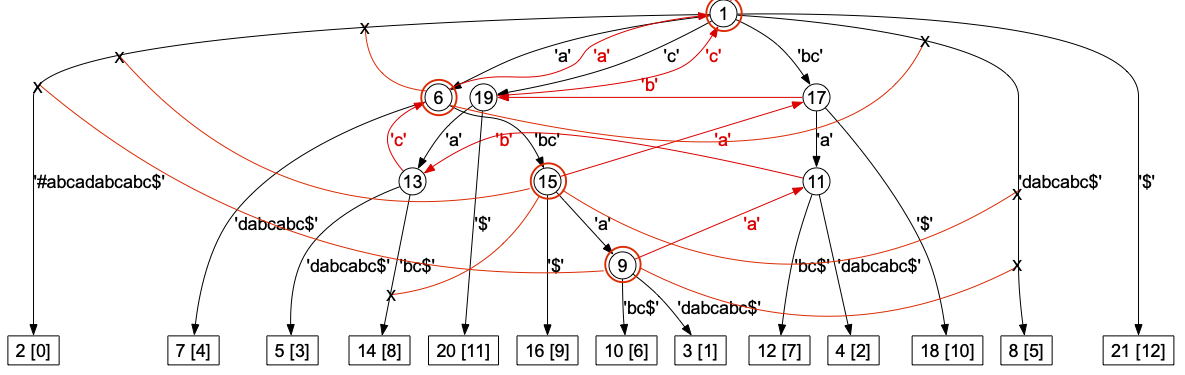
\includegraphics[width=1.00\textwidth]{fig/exp1/fwdstree_org.png}
%% \smallskip
%% \caption{
%%   Illustration of search strategies for maximal repeat enumeration on a string
%%   $S = \mathtt{\#abcadabcabc\$}$ of \cref{tbl:arrays}. 
%%   %S=#abcadabcabc$.
%%   The figure shows the suffix tree (black) and Winer tree (red) of $S$, highlighting maximal repeats with red double circles. Nodes represent right-branching substrings labeled with its SA-range, and edges are labeled with strings (black) or characters (red). Previous methods $\BUSA$ and $\TDBW$ traverse entire subtrees, while our method $\MREnum$ efficiently traverses only relevant red nodes via black edges, significantly reducing the search space.
%% }\label{fig:fwdstree}
%% \end{figure}
%% %%%%%%


%% %%%%%%%%

%% \textbf{Previous work}.\ 
%% %%%%%
%% The current best upperbounds on the runtime of enumerating all distinct  maximal repeats were summarized as the following algorithm schema (see \cref{fig:fwdstree}).
%% The first scheme is abbreviated as \BUSA{} (bottom-up search with the suffix array),  and the best runtime was $O(n)$ time using $O(n)$ words of space based on $SA$, $ISA$, and the RMQ structure on $LCP$, shown by Narisawa, Inenaga, Bannai, and Takeda~\cite{narisawa2007efficient}. 
%% The second scheme is abbreviated as \TDBW{} (top-down search with the Burrows-Wheeler Transformation/BWT), and the runtime was $O(n \log\sigma)$ time using $O(n/\log_\sigma n)$ words of space based on the Wavelet tree on $BWT$, shown by Beller, Berger, and Ohlebusch~\cite{beller:berger2012space:efficient:bbo}.
%% %%where $ISA$ is the inverse $SA$, and $LCP$ is the longest common prefix array of the string.
%% After these seminal work with \textit{uncompressed indexes}~\cite{narisawa2007efficient,beller:berger2012space:efficient:bbo}, there have been a few recent researches on repetition-aware enumeration of maximal repeats with \textit{compressed indexes}~\cite{belazzougui2020linear,nishimoto:cpm2021enum}. For example, Nishimoto and Tabei~\cite{nishimoto:cpm2021enum} have nicely reduced the space to $O(r(S))$ with polylogarithmic factor retaining $O(n)$ time based on a variant of the \textit{$r$-index}. However, to the best of our knowledge, there have been no results that simutaneously achieve sublinear space and time sensitive to repetition parameters including $r(S), z(S)$, or $e_R(S)$. 


%% %%%%%%% tblnew.tex
%% %%% tabnew.tex
%% %\centering
%% \begin{table}[t]
%%   \caption{%
%%     Summary of the time and space of the previous and proposed algorithms for enumeration of all distinct maximal repeats in a string $S$ of length $n$,
%%     %of maximal repeats,
%%     %% where $\sigma$ is the alphabet size,
%%     %% $r$ is the number of BWT runs,
%%     %% $e_R$ is the number of right-extensions,
%%     %% %of maximal repeats,
%%     where
%%     $\sigma$, $r$, and $e_R$ are the numbers of 
%%     characters, BWT runs, and right-extensions, respectively, 
%%     $\delta$ is the substring complexity of $S$.
%%     See \cref{sec:prelim:ds:array} for abbreviations in column \textit{Data structure}, and BU/TD and SA/BW indicate bottom-up/top-down search and SA/BWT arrays, respectively, in \textit{Scheme}.
%% }\label{table:summary:new}
%% %%%% 
%% \medskip
%% \begin{minipage}{\textwidth}
%% %\hspace{-1.2em}
%% \begin{tabular}{%
%% p{.0em}%1margin
%% p{7.6em}%2algo
%% p{10.0em}%3underlying
%% >{\centering}p{7em}%5time
%% %>{\centering}p{8.5em}%6indexspace
%% >{\centering}p{8.5em}%%6indexspace
%% p{3.0em}%4type
%% %c%7dammy
%% %>{}p{4.9em}%7dammy
%% }\toprule
%%   & Algorithm
%%   & Data Structure	
%%   %% & Underlying\break Structure	
%% %% & Index Space
%% & Space (words)
%% & Enum.~Time 
%% & Scheme \\
%% %%%%
%% \midrule 
%% %% \multicolumn{6}{l}{Existing array-based algorithms} \\
%% & Narisawa~\cite{narisawa2007efficient}	&
%% \textsc{Sa,\,Isa,\,Txt,\,Lcp}\cite{manber:myers1993suffixarrays} & $O(n)$	& $O(n)$ & \BUSA{} 	 \\
%% %% & Narisawa~\cite{narisawa2007efficient}	& SA\cite{manber:myers1993suffixarrays} & $O(n)$	& $O(n)$ & \BUSA{} 	 \\
%% %% & Okanohara+~\cite{okanohara2009text}	& SA\cite{manber:myers1993suffixarrays}\&FM\cite{Ferragina05:FM} & $O(n)$& $O(n\log\sigma)$	 & \bufwd 	 \\
%% & Beller+~\cite{beller:berger2012space:efficient:bbo} 	&
%% \textsc{Bwt,\,Wt}~\cite{Ferragina05:FM}
%% & $O(n/\log_\sigma n)$ & $O(n\log\sigma)$	& \TDBW{} \\
%% & Belazzougui+\cite{belazzougui2015space:unusual} 	&
%% \textsc{Bwt,\,Rdq}~\cite{belazzougui2020linear}
%% & $O(n/\log_\sigma n)$ & $O(n)$	& \TDBW{} 	 \\
%% %% & Belazzougui+\cite{belazzougui2020linear} 	& Belazzougui+\cite{belazzougui2020linear} & $O(n)$ & $O(n)$	& \TDBW{} 	 \\
%% %% & Belazzougui+\cite{belazzougui2020linear} 	& Belazzougui+\cite{belazzougui2020linear} & $O(n\log n\log\sigma)$ & $O(n)$	& \TDBW{} 	 \\
%% & Nishimoto+~\cite{nishimoto:cpm2021enum} 	& Gagie+~\cite{gagie:navarro:prezza2020fully} & $O(r\log({\frac n r})\log n)$ & $O(n\polylog n)$ & \TDBW{} 	 \\
%% %%%%%
%% %% \multicolumn{6}{l}{Proposed algorithms} \\
%% \\
%% & [This paper]	&
%% \makebox[11em][l]{\textsc{Sa,\,Isa,\,Txt,\,Rmq$_\textsc{LCP}$}\!\cite{manber:myers1993suffixarrays}}
%%  & $O(n)$ & $O(e_R)$	& \MREnum	 \\
%% %% & [This paper]	& SA\cite{manber:myers1993suffixarrays} & $O(n)$ & $O(e_R)$	& \MREnum	 \\
%% & [This paper]   	& Gagie+~\cite{gagie:navarro:prezza2020fully}	 	& $O(r\log({\frac n r})\log n)$ & $O(e_R \log({\frac n r}))$& \MREnum \\
%% & [This paper]   	& $\delta$-SA~\cite{kempa:kociumaka2023collapsing}  & $O(\delta\log({\frac n \delta}) \log n)$	& $O(e_R \log^{4+\eps}(n))$	 & \MREnum  \\
%% \bottomrule
%% \end{tabular}
%% \end{minipage}
%% \end{table}
%% %%%%%%%

%% %% In particular, we are interested in the complexity of enumerating maximal repeats for highly-repetitive strings, in terms of repetition measures, which take smaler values than the length $n$ of a string. For instance, collections of human genome sequences with small pertabations and Wikipedia documents with edit history are examples of highly-repetitive strings. In highly repetitive strings, a number of measures of repetition growing sublinearly in the length of the string. Particularly, we focus on the repetition measure $e_R(S)$ associated to maximal repeats, introduced by Belazzougui \textit{et al.}~\cite{belazzougui:cunial:gagie:prezza:raffinot2015composite} in 2015, where $e_R(S)$ is the number of right-extensions of maximal repeats in a string~$S$. It is shown by~\cite{belazzougui:cunial:gagie:prezza:raffinot2015composite} that the measure $e_R$ is lowerbounded by other well-known repetition measures $r(S)$ and $z(S)$, the number of runs in the BWT and the number of LZ-phrases of $S$, respectively. 

%% %In this paper, we prove the following theorem.
%% %% To overcome this problem, we propose a simple and faster algorithm with a novel search strategy, which has not been examined so far by the previous work~\cite{narisawa2007efficient,beller:berger2012space:efficient:bbo,belazzougui2020linear,nishimoto:cpm2021enum}.  
%% %% We prove the following theorem.
%% %% To overcome this problem, we propose a simple and faster algorithm scheme, abbreviated \MREnum (top-down search with the suffix array), with a novel search strategy, which has not been examined so far by the previous work~\cite{narisawa2007efficient,beller:berger2012space:efficient:bbo,belazzougui2020linear,nishimoto:cpm2021enum}.  

%% \textbf{Goal of research and main results}.\ 
%% %%%%%
%% To overcome this problem, we propose a novel search scheme, abbreviated as \MREnum{} (top-down search with the suffix array), suitable for simple and faster algorithms, which has not been examined so far by the previous work~\cite{narisawa2007efficient,beller:berger2012space:efficient:bbo,belazzougui2020linear,nishimoto:cpm2021enum}.  
%% We prove the following theorem.

%% %% \begin{trivlist}\item[] \textbf{\cref{thm:algo:main}}
%% %%   Let $S$ be a string of length $n$ over an alphabet of $\sigma\ge 2$ symbols.  We assume any data structure that stores $S$ in $s_\fn{acc}(n)$ words of space supporting (i) access to $SA[i]$ and $ISA[i]$, and (ii) $RMQ_{LCP}(L, R)$ on $LCP$ in $t_\fn{acc}(n)$ worst-case time.
%% %% Then, all of distinct maximal repeats in $S$ can be enumerated in $O(e_R\cdot t_\fn{acc}(n))$ time and $O(\sigma^2 \log e_R)$ words of working space, where $\mu$ is the number of distinct maximal repeats in $S$ and  $e_R$ is the number of the right-extensions of maximal repeats such that $\mu \le e_R \le n$. 
%% %% \end{trivlist}

%% \begin{theorem}[main result]\label{thm:algo:main}
%%   Let $S$ be a string of length $n$ over an alphabet of $\sigma\ge 2$ symbols.
%%   We assume any data structure that stores $S$ in $s_\fn{acc}(n)$ words of space supporting (i) access to $SA[i], ISA[i]$, and $S[i]$, and (ii) $RMQ_{LCP}(L, R)$ on $LCP$ in $t_\fn{acc}(n)$ worst-case time.
%% Then, all of distinct maximal repeats in $S$ can be enumerated in $O(e_R\cdot t_\fn{acc}(n))$ time and $O(\sigma^2 \log e_R)$ words of working space, where $\mu$ is the number of distinct maximal repeats in $S$ and  $e_R$ is the number of their right-extensions such that $\mu \le e_R \le n$. 
%% \end{theorem}

%% By substituting different SA index for \cref{thm:algo:main} above, we obtain a variety of enumeration algorithms for distinct maximal repeats with different time and space trade-offs.
%% In \cref{table:summary:new}, we show the summary of results. 
%% %% 
%% Firstly, we observe the case with the uncompressed SA index of Manber and Myers~\cite{manber:myers1993suffixarrays}, and the RMQ structure $RMQ_{LCP}$ on $LCP$ by Bender and Colton~\cite{bender:colton2000thelcaproblem}. 

%% \begin{theorem}\label{thm:algo:uncompressed:sa}
%%   All distinct maximal repeats in a string $S$ of length $n$ can be enumerated in $O(e_R)$ time and $O(\sigma^2 \log n)$ working space based on $SA, ISA, S$, and $RMQ_{LCP}$ using $O(n)$ words of space. 
%% \end{theorem}

%% Secondly, we observe the cases with the repetition-aware, compressed SA indexes, namely,
%% the \textit{$r$-index} with $O(r\polylog(n))$ space by Gagie \textit{et al.}~\cite{gagie:navarro:prezza2020fully}, and
%% the \textit{$\delta$-spaced SA index} with $O(\delta\polylog(n))$ space by Kempa and Kociumaka~\cite{kempa:kociumaka2023collapsing}, where $\delta \le r \le e_R$ (see \cite{kociumaka:navarro:olivares2024near:delta:optimal,kempa2018roots,belazzougui:cunial:gagie:prezza:raffinot2015composite}).
%% Then, we obtain enumeration algorithms with $O(e_R\polylog(n))$ runtime and space simultaneously shown in the last two lines of \cref{table:summary:new} (\cref{thm:applications}, \ref{item:result:bidirect:index}--\ref{item:result:compressed:delta:index}). 
%% If $e_R = o(n/\log^c n)$ for $c\ge 1$ and $c\ge 4+\eps$, respectively, for hightly-repetitive strings (e.g., Fibonacci or Thue-Morse words~\cite{radoszewski:rytter2012structure:cdawg:thuemorse}), these results yield the first sublinear time and space MR enumeration. 


%% \textbf{Contributions}.\ 
%% %%%%%
%% In this paper, we presented a simple and modular algorithm for enumerating all distinct maximal repeats by using $SA$ and associated auxiliary structures as black box.
%% Technically, the key to our results with time and space complexities that are  sensitive to the repetitiveness measure $e_R$ is a simple and modular algorithm with a novel search strategy (see \cref{fig:fwdstree}), which has not been used before for this problem. 
%% Overall, this work presents the first sublinear, repetitiveness-aware algorithms for highly repetitive strings.

%% %% To overcome the difficulties of the previous approaches, we propose a simple and faster algorithm with a novel search strategy, which has not been examined so far by the previous work~\cite{narisawa2007efficient,beller:berger2012space:efficient:bbo,belazzougui2020linear,nishimoto:cpm2021enum}

%% %% \begin{toappendix}
%% %% We discuss the following applications. 
%% %% In addition to maximal repeats, much attention has been paid to other string patterns in bioinformatics such as minimal absent words (MAWs)~\cite{barton2014linear}, minimal unique substrings (MUSs)~\cite{ilie2011minimum}, and their generalization called minimal rare words (MRWs)~\cite{belazzougui2015space:unusual}. We also focus on these string patterns because they are closely related to maximal repeats~\cite{inenaga2024computing}.
%% %% For applications, our algorithm significantly improves the running times of the previous $O(n)$-time algorithms~\cite{barton2014linear,ilie2011minimum,belazzougui2015space:unusual} based on the suffix array $SA$ with auxiliary structures, for sequence patterns including MAWs, MUSs, and MRWs related to maximal repeats. We also discuss application of our algorithm to faster construction of the CDAWG string index with $SA$. 
%% %% \end{toappendix}

\textbf{Organization of this paper}.\ 
%%%%%
\cref{sec:prelim} introduces basic notions and definitions, necessary to the rest of this paper. 
%% \cref{sec:prev} gives a brief review on the previous approaches in maximal repeats enumeration.
In \cref{sec:mrep} and \cref{sec:algo}, we first present a basic algorithm for enumerating the set $\MR(S)$ of all of $occ$ maximal repeats of a string $S$ over alphabet $\Sigma$ can be enumerated in $O(e_R + occ)$ time and $O(e_L  + |\Sigma|^2 \log n)$ working space, where $n$ is the length of $S$. 
In \cref{sec:mrw}, we extend the basic algorithm to afoementioned classes of unusual words, and show that the set of all patterns of a string $S$ within any of these classes can be enumerated in $O(e_L + e_R + occ)$ time, and give its correctness and computational complexity.
In \cref{sec:conc}, we conclude. 


%% approach

\section{Review of Previous Algorithms}
\label{sec:review}

Before presenting our algorithm, we start with reviewing existing approaches for maximal repeat enumeration. 



%%%%%% %% fig:CDAWG
\begin{figure}[t]
  \centering
  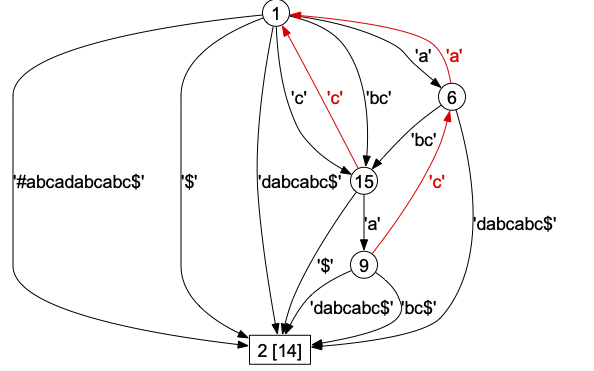
\includegraphics[height=0.4\textwidth]{fig/exp1/cdawg.png}
  %% 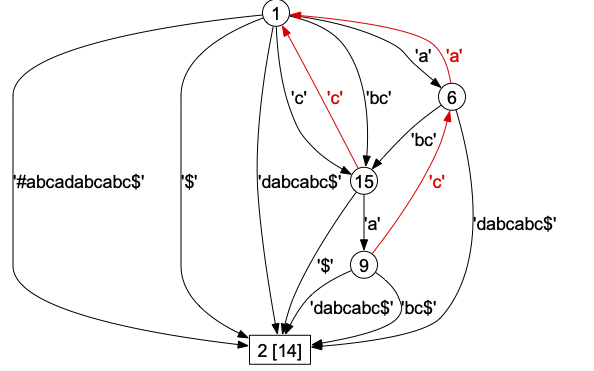
\includegraphics[height=0.4\textwidth]{fig/exp1/cdawg.pdf}
  \medskip 
  \caption{The CDAWG for a text $T = \mathtt{\#abcadabcabc\$}$ of length $13$. Its branching nodes $1, 6, 15$, and $9$ represents all of four maximal repeats $\eps, \mathtt{a}, \mathtt{abc}$, and $\mathtt{abca}$ with frequencies $14, 4, 3$, and $2$, respectively.
  }\label{fig:cdawg}
\end{figure}
%%%%%%


\subsection{Basics of enumerating maximal repeats}
Firstly, we explain the basic strategy of maximal repeat enumeration, which are common to all existing algorithms. 
Our result is obtained by combination of the top-down traversal of the virtual affix tree and efficient test for the left-branchingity based on the suffix array of a text. 
%%% 
We briefly explain our approach in the followings. 
%%We made a through survey of the existing algorithms for MR-enumeration. 

The CDAWG $\sig G$ for a txt $T$ (see \cref{fig:cdawg}) is a central data structure for dealing with  maximal repeats. It can be obtained from the suffix tree $\sig S$ (or equivalently its Weiner tree $\sig W$) for the same $T$ by merging all isomophic subtrees. Actually, what Raffinot~\cite{raffinot2001maximal} found was that that all nodes but the sink of the resuting DAG $G$, i.e., the CDAWG, represent all maximal repeats. 

On the other hand, if we view from the side of the suffix tree, all of its nodes with branching (outgoing) forward edges represent right-branching subwords of $T$, while all nodes with branching (incoming) backward edges (suffix links) represent left-branching subwords of $T$. Since maximal repeats are those subwords which are both left- and right-branching, we seek them by traversing either $\sig S$ or $\sig W$. 

Based on the above observation, we can classify enumeration algorithms by the following g two criteria: 
\begin{enumerate}[(1)]
\item The \textit{direction} of the traversal, i.e., either \textit{top-down} from the root to leaves~(\td), or \textit{bottom-up} from leaves to the root~(\bu). 
\item The \textit{types of edges} to follows, i.e., either \textit{forward}~(\fw) or \textit{backward}~(\bw). 
\end{enumerate}

\subsection{Classification of existing algorithms}

In \cref{table:summary}, we list and classify the state-of-the-art methods for MR enumeration ~\cite{narisawa2007efficient,okanohara2009linear,beller:berger2012space:efficient:bbo,belazzougui2020linear,nishimoto:cpm2021enum}. In the table, the last column ``Trav.~Type'' indicates the classification in combinations of tokens, such as $\tdfw$, the first one from $\set{\td, \bu}$ and the second one from $\set{\fw, \bw}$. 

By careful look at \cref{table:summary}, we found the existing algorithms fall into three groups below: 
\begin{enumerate}[(I)]
\item Three graph-based algorithms with type \tdfw, which has as an underlying structure either the suffix tree $\sig S$ or the CDAWG $\sig G$. 
There are no array-based algorithms with type \tdfw. 

\item Three array-based algorithms with type \tdbw, which has as an underlying structure is the Weiner tree $\sig W$. They traverse $\sig W$ based on the top-down simulation method proposed by Abouelhoda~\cite{abouelhoda2004replacing} using the BWT array and Wavelet tree. 


\item Two array-based algorithms with type \bufw, which has as an  underlying structure the suffix tree $\sig S$. They traverse $\sig S$ based on the bottom-up simulation method proposed by Kasai et al.~\cite{kasai:lee2001lcp:linear} 
using the SA and LCP arrays. 
\end{enumerate}

From the above classification, we can obtain some useful observation about the possible design of an efficient enumeration algorithm for MRs. 

\subsection{Analysis of the existing approaches}
%\subsection{Lessons learnt}
Firstly, all existing algorithms in group (I) are graph-based ones. Thus, they directly traverse the graph top-down by following forward edges without any difficulty. 
If the underlying graph $\sig G$ is isomorphic to the CDAWG of $T$, they can run in $O(e_R)$ time as desired. We can also see that there have been no existing array-based algorithms with type $\tdfw$ so far. We will come back to this issue later. 

Next, all existing array-based algorithms fall into the cases (II) and (III). 
For the case (II), algorithms has type \tdbw. They suffer from the fact that the underly tree $\sig W$ consists only of atomic backward edges. Therefore, the algorithms must traverse atomic backward edges one by one using the LF-mapping. From this reason, they must consume $\Theta(n)$ time by following a long chain of non-branching nodes until they  encounter a maximal repeat. 

For the case (III), algorithms has type \bufw. Unlike case (II), since all forward edges in the suffix tree $\sig S$ are path-compressed, they can avoid the problem with atomic edges. However, due to the bottom-up direction, they cannot make branch-and-bound search by pruning the useless subtrees. Consequently, they must travperse all of $\Theta(n)$ edges, resulting $\Theta(n)$ total running time. 

Finally, we are curious about this fact because we could not find any immediate reason by which we should avoid using the combination {\tdfw}, namely, the \textit{top-down search of the suffix tree $\sig S$ following forward edges}.  
Next, we will examine this approach further. 

\subsection{Our approach}
From the discussion in the previous subsection, the search strategy {\tdfw} seems a novel approach for efficient enumeration of maximal repeats. Actually, we can observe the following reasons to employ {\tdfw} as the basic strategy of our enumeration algorithm:  
\begin{enumerate}
\item \textit{Efficient pruning of non-maximal nodes}. Top-down search direction seems suitable to prune useless search paths than bottom-up search direction. This pruning should be efficiently done based on the left- or right-branchingity tests on indivisual nodes or subwords. This can be done by using the combination of the SA and LCP arrays with the help of the RMQ structure. 

\item \textit{Avoiding traversal of atomic edges}. Traversal with forward edges in $\sig S$ seems preferrable than that on backward edges in $\sig W$ to avoid traversal of atomic edges symbol by symbol. Since the path compression is closely related to the longest common prefixes of suffixes containing the locus of a subword, efficient test can be supported by  the LCP array with the RMQ structure, again. 
\end{enumerate}

We explain these ideas in the next section. 

%%% EOF

%% \input{review}
%% algo.tex
%% \section{The Proposed Algorithm}
\section{A Simple and Faster Algorithm}
\label{sec:algo}
%%%% 
Now, we present our $O(e_R)$-time algorithm scheme $\TDSA$ (\textit{top-down search with the suffix array}) for enumerating all distinct maximal repeats of a string $S$,  based on $SA$, $ISA$, $S$, and the RMQ structure on $LCP$ of a text $S$ using $O(n)$ words of space, where $e_R \le n$ is the measure of repetitiveness of a text, namely, the number of right-extensions.


%%%%%%%%%%%%%%%%%
{
  \setlength{\interspacetitleruled}{0pt}%
  \setlength{\algotitleheightrule}{0pt}%  
  \begin{algorithm}[h]
  %% \caption{Top-down MR-enumeration algorithm with SA}\label{algo:maxrep:tdfw}
  \textbf{Procedure} \TDSA$(\tau_0 = ([L_0..R_0], \ell_0))$:\\
  %%\KwGiven{}
  %% \KwIn{The triple $\tau_0 = (L_0, R_0, \ell_0)$ for a right-branching substring $X$ of a text.}
  %% \KwOut{}
  \Begin{
      \textbf{output} $\tau_0$
      \Comment*{A maximal repeat is found}
      \For %(\CM{})
           {child $\tau = ([L..R], \ell)$ of the parent $([L_0..R_0], \ell_0)$}{
          \Comment{It is ensured that $R - L \ge 1$ and $\tau$ is right-branching}
          Decide if $\tau$ is left-branching by $SA, ISA$, and $S$ (\cref{lem:leftmaximal:character})\; 
          \If {$\tau$ is left-branching}{          
            \TDSA$(\tau)$\; 
          }
        }
  }
  \end{algorithm}
}  
%%%%%%%%%%%%%%%%%

\subsection{Search strategy}
\label{sec:algo:tdsa}
%%%% 
A basic idea of $\TDSA$ is the use of \textit{top-down search} using the forward search for right-extensions based on the \textit{suffix array}, unlike the backward search for right-extensions adopted by \TDBW.
This enables the sound and early pruning of hopeless right-extensions that never become left-branching ones.
%% 
Now, we define the parent-child relation over triples related to the suffix tree of $S$ as follows. For triples $\tau_0 = ([L_0..R_0], \ell_0)$ and $\tau = ([L..R], \ell)$ defining strings $U$ and $W$, $\tau$ is called the \textit{$b$-child} of $\tau_0$ if $W = Ub$ for some character $b \in \Sigma$, called a \textit{branching character}. The ancestors and descendants of $\tau$ are defined in the standard manner.
%%We have. 

\begin{lemma}\label{lem:prune:leftbranch}
Suppose that a triple $\pi$ is an ancestor of a triple $\tau$. If the substring defined by $\tau$ is left-branching, the substring defined by $\tau$ is also left-branching. 
\end{lemma}

Recall that a repeat is maximal if and only if it is both left- and right-maximal in $S$. Lemma~\cref{lem:prune:leftbranch} says that the set $MR(S)$ occupies the \textit{upper connected region} of the suffix tree of $S$. For instance, we see in \cref{fig:fwdstree} that $MR(S)$ occupies the node sets $\set{1,6,15,9}$. 
%% In other words, if a triple $\tau$ is not left-branching, then any of its ancestor is also not left-branching.
This implies the next rule.

\begin{itemize}\item[]
\quad\textsc{Pruning rule}: {Every non-left-branching triple is pruned.}
\end{itemize}

For testing the left-branching property, we use the following lemma, which is a slight modification of Narisawa \textit{et al.}~\cite[Lemma~10]{narisawa2007efficient}. 

%% \begin{lemma}\label{lem:leftmaximal:character}
%% Let $W$ be any substring of $S$ and $\tau = (L,R, \ell)$ be the triple defining~$W$. 
%% Then,
%% %% the following conditions (1)--(3) are equivalent each other: 
%% (1) $W$ is not left-branching in $S$ if and only if  
%% (2) $(R - L + 1) = (ISA[SA[L]-1] - ISA[SA[R]-1] + 1)$. 
%% \end{lemma}

\begin{lemma}[Narisawa \textit{et al.}~\cite{narisawa2007efficient}]\label{lem:leftmaximal:character}
For the triple $\tau = (L,R, \ell)$ for any substring~$W$ of $S$, 
(1) $W$ is not left-branching in $S$ if and only if  
(2) (i) $S[p-1] = S[q-1]$ and (ii) $R - L = \id{ISA}[p-1] - \id{ISA}[q-1]$ with $p = SA[L]$ and $q = SA[R]$.
\end{lemma}

\begin{proof}
%%We add clause (*)  
We let $p = SA[L], q = SA[R]$. 
$(1)\Implies (2)$: Suppose that $W$ is not left-branching in $S$.
Then, all occurrences of $W$ in $S$ have the same previous characters $c \in \Sigma$ in $\spos(W)$. Thus, it immediately follows that $BWT[L, R]$ is monotone.
Let $\varphi: k \mapsto ISA[SA[k]-1]$. By observing $\varphi$ coincodes to the LF-mapping~\cite{Ferragina05:FM}, claim (2) immediately follows. 
%%% 
$(2) \Implies (1)$: 
%We show the contraposition $\neg (1) \Implies \neg (2)$. 
Suppose (2), and to contradict that $\neg$(2) $W$ is left-branching in $S$. Let $I = [L..R]$. Then, there exist a pair of preceding characters $c = S[p-1], d=S[q-1]$ with $c\not= d$ for some $p, q \in \spos(W)$. It follows that $\varphi$ transforms the positions in  $SA[L..R]$ into at least two, mutually disjoint, non-empty ranges $I_c, I_d$ with $I_c\uplus I_d = I$ starting with $c$ and $d$, respectively. By assumption (2.i), we see that positions $SA[L]$ and $SA[R]$ move into the same range, say $I_c$ with $L_c := \varphi(L)$ and $R_c := \varphi(R)$ as the left and right ends of $I_c$ since $\varphi$ preserves $<_\lex$. 
Since both of $I_c$ and $I_d$ are non-empty, we have $R_c - L_c + 1 = |I_c| < |I| = R - L + 1$; contradiction to assumption (2.ii). By contradiction, we conclude condition (1) holds. 
\qed   
\end{proof}

%% \begin{proof}
%% We add clause (*)  $BWT[L, R]$ is monotone. 
%% We let $p = SA[L], q = SA[R]$. 
%% $(1)\Implies (*)$: Suppose that $W$ is not left-branching in $S$. Then, we see that all occurrences of $W$ in $S$ have the same character, say $c$, in the previous positions in $\spos(W)$. Thus, the claim (*) immediately follows. 
%% %%% 
%% $(*) \Implies (2)$: We can easily observe that the function $f(k) := ISA[SA[k]]$ realizes the LF-mapping~\cite{Ferragina05:FM} by definition. Hence, claim (2) immediately follows from (*). 
%% %%% 
%% $(2) \Implies (1)$: 
%% %We show the contraposition $\neg (1) \Implies \neg (2)$. 
%% Suppose that $W$ is left-branching in $S$. Then, it follows that $c = S[p-1]\not= S[q-1] = d$ for some $p, q \in\spos(W)$ of $W$. 
%% %It follows that the subarray $BWT[L,R]$ contains mutually distinct $c$ and $d$. Since $[L,R]$ is the SA-interval of $W$, 
%% Therefore, the substring $W$ has a pair of distinct characters $c = S[p-1]$ and $d = S[q-1]$ at the previous positions of its start positions. By contraposition, $W$ is left-branching. 
%% Combining the above arguments, the lemma is proved. 
%% \qed   
%% \end{proof}

\subsection{Computing the set of child triples}
\label{sec:algo:branch}
%%%% 
%% An SA-range $[L..R]$ is called an $\ell$-range if it satisfies the conditions (i)--(iv) below: 
%% \begin{enumerate*}[(i)]
%% \item $LCP[L] < \ell$, 
%% \item $LCP[L] \ge \ell$ for all $k \in [L+1..R]$, 
%% \item $LCP[L] = \ell$ for at least $k \in [L+1..R]$, and 
%% \item $LCP[R+1] < \ell$.  
%% \end{enumerate*}
An SA-range $[L..R]$ is called an \textit{$\ell$-range} if the lcp of all suffixes starting  with positions in $SA[L..R]$ equals~$\ell$, i.e.,
$\ell = \min\sete{ SA[k] \mid k \in [L+1..R] }$. 
Then, an index $k \in [L+1..R]$ is called a \textit{$\ell$-index} if it achieves the lcp-value $\ell$, i.e., $LCP[k] = \ell$.
Cosider the suffix tree $\sig T$ of a string $S$.
%% We say that a triple $\tau = ([L..R], \ell)$ is a child of triple $\tau_0 = ([L_0..R_0], \ell_0)$ 
If triples $\tau_0$ and $\tau$ represent string labels of a node $u$ and its child $w$ in the suffix tree (see gusfield1997book:stree), we say that the range $[L..R]$ is a \textit{child} of the range $[[L_0..R_0]]$. 
%% 
For computing the set of child ranges of a given $\ell$-range $[L_0, R_0]$, we use the following lemma.

\begin{lemma}[Abouelhoda, Kurtz, and Ohlebusch~\cite{abouelhoda2004replacing}]\label{lem:child:ranges}
  Let $[L_0, R_0]$ be any $\ell$-range.
  If $M_1 < M_2 < \dots < M_k$ are the $\ell$-indexes in ascending order, then the child ranges of $[L_0, R_0]$ are
  $[L_0..M_1-1], 
   [M_1..M_2-1], 
   \ldots,
   [M_k..R_0]$.  
\end{lemma}

Although Abouelhoda \textit{et al.}~\cite{abouelhoda2004replacing} presented based on \cref{lem:child:ranges} how to use an array $\op{childtab}[1..n]$ of cells with three integer fields $\op{up}, \op{down}$, $\op{nextIndex} \in [n]$ for traversing the virtual suffix tree top-down, the method is not suitable to our purpose. 
%%% 
Instead, combining \cref{lem:child:ranges} above and the recursive procedure for colored range query by Muthukrishnan~\cite{muthukrishnan2002efficient} (see also the textbook by Ohlebusch~\cite{ohlebusch2013bookbioinfo}), we present a recusive procedure \proc{BranchRepeats} for enumerating the set of all child ranges of an $\ell$-range below, invoked in the top-level as \proc{BranchRepeats}$([L..R], \ell_*)$ with $\ell_* = RMQ_{LCP}(L+1, R)$. 

%%%%%%%%%%%%%%%%%
{
\setlength{\interspacetitleruled}{0pt}%
\setlength{\algotitleheightrule}{0pt}%  
\begin{algorithm}[h]
  \textbf{Procedure} \proc{BranchRepeats}$([L..R], \ell_*)$:\\  
  \Begin{
      \If {$R - L \ge 1$}
      {
        $(M, \ell) \gets RMQ_{LCP}(L+1, R)$
        \Comment*{$\ell = LCP[M]$}
        \iIf {$\ell_* < \ell$}{
          \textbf{output} $(L, R, \ell)$
          \Comment*{$[L,R]$ is monotone}
        }
        \Else  (\CM{$\ell_* = \ell$} and $[L,R]$ is diverse) 
        {
          $\proc{BranchRepeats}([L..M-1], \ell_*)$\; 
          $\proc{BranchRepeats}([M..R], \ell_*)$\;
        }
      }
  }
\end{algorithm}
}
%%%%%%%%%%%%%%%%%

By using the RMQ structure on $LCP$ that supports constant time queries, the procedure correctly computes the answers in output-sensitive manner. 


\begin{lemma}[Muthukrishnan~\cite{muthukrishnan2002efficient}, Ohlebusch~\cite{ohlebusch2013bookbioinfo}]
  The set of all child ranges of an $\ell$-range $[L..R]$ can be enumerated in $O(k)$ time in $O(n)$ space
  using $RMQ_{LCP}$, 
%% using the RMQ structure on $LCP$, 
where $k$ is the number of the child renges to output.  
\end{lemma}


%%%%%%%%%%%%
\subsection{Execution example}

In \cref{fig:run:example}, we show an example run of Algorithm $\TDSA$ for a text $S[0..10] = \mathtt{\#aabaababb\$}$. The black and red trees, respectively, indicate the suffix and the Weiner trees of $S$. Each circle indicates a node with the string label and the triple. A gray node corresponds a maximal repeat. 
We observe that the proposed algorithm $\TDSA$ only traverses the suffix tree starting from the root, and enumerates all maximal repeats, by visiting all and only the gray nodes. 


%%%%%%%%%%%%
\subsection{Complexity Analysis}
%%%%%
As the main result, we show \cref{thm:algo:main}, 
combining Lemmas~\ref{lem:prune:leftbranch},
\ref{lem:leftmaximal:character}, and 
\ref{lem:child:ranges}.
%% \cref{lem:prune:leftbranch},
%% \cref{lem:leftmaximal:character}, and 
%% \cref{lem:child:ranges}.

%% \begin{trivlist}\item[]
%% (\textit{The proof for \cref{thm:algo:main}})\quad   
%% \begin{proof}
\begin{statement}{The proof for \cref{thm:algo:main}}
  From \cref{lem:prune:leftbranch}, we observe that any maximal repeat (MR) $W \in MR(S)$ is either (i) the empty string $\eps \in MR(S)$, where $|\Sigma|\ge 2$, or (ii) there exists a shorter MR $U \in MR(S)$ and a $b \in \Sigma$ exactly when (ii.a) $W = \rext{Ub}$ and (ii.b) $\lext{W} = W$.
  By \cref{lem:child:ranges}, we can obtain such a $b \in \Sigma$ in (ii.a), and by \cref{lem:leftmaximal:character}, we can make test in (ii.b) in $O(1)$ time. 
  Combining the above arguments, the correctness and time complexities follows. 
  %%% 
  To bound the working space, we use the technique by Belazzougui \textit{et al.}~\cite[Lemma~4.2]{belazzougui2020linear} as follows. Consider the suffix tree $\sig T$ of $S$ as the search tree of our algorithm. At each iteration in the top-down traversal, we first select the child with the widest SA-range, having the largest number of leaves. Since this generetes the heavy-leaf decomposition of $\sig T$, the modified traversal yields at most $O(\log n)$ levels with $O(\sigma^2)$ side information per level, each has $O(1)$ size in $\sig T$. This leads to the working space of $O(\min\set{e_R, \sigma\log n}) = O(\sigma^2\log n)$ words. \qed 
\end{statement}

%%%%%%
\begin{figure}[t]
  \centering
  \rule{0.09\textwidth}{0em}
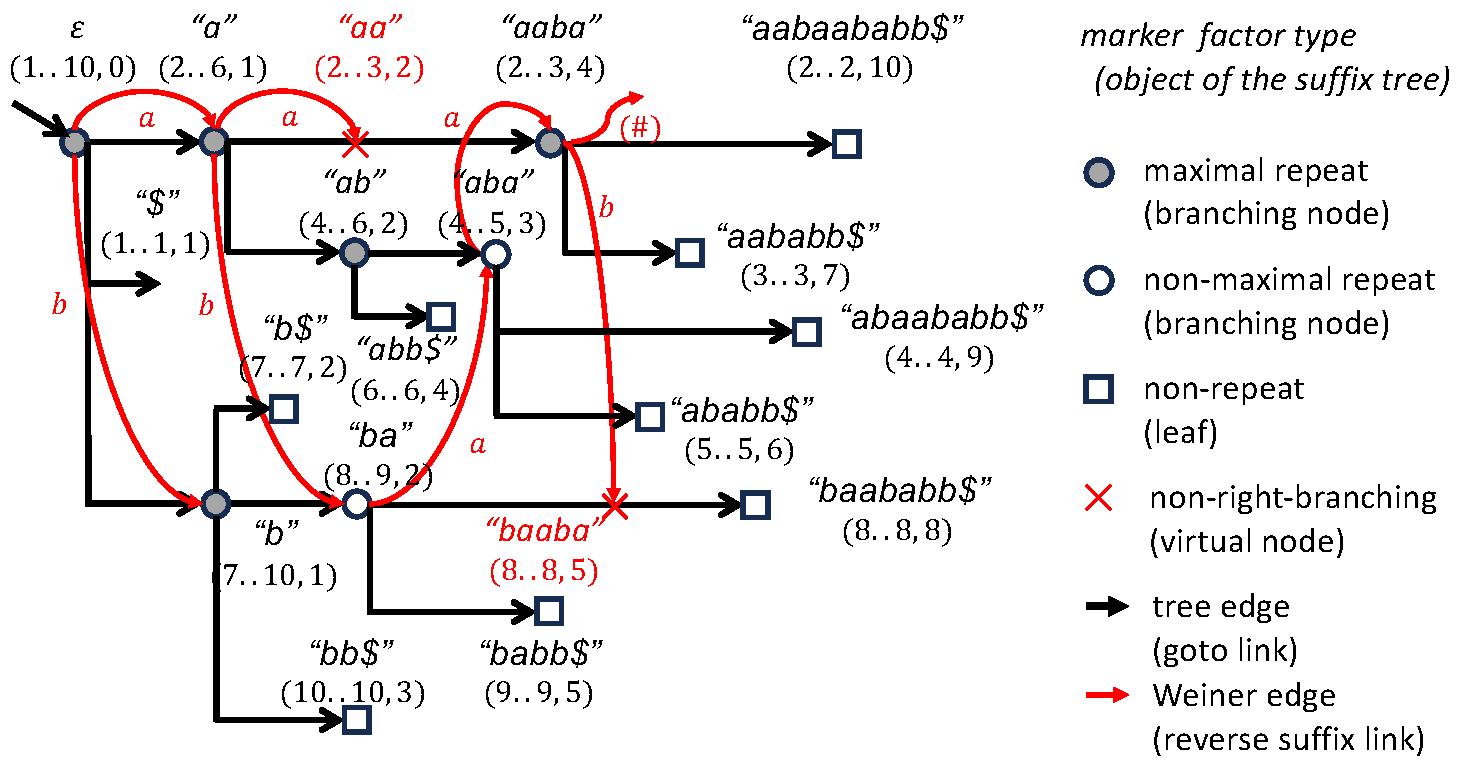
\includegraphics[width=0.9\textwidth]{fig2.pdf}
\vspace{.75\baselineskip}
\caption{An example run of Algorithm $\TDSA$ for a text $S = \mathtt{aabaababb\$}$, where the left endmarker $S[0]=\#$ and the related suffixes are omitted. 
}\label{fig:run:example}
\end{figure}
%%%%%%

%% %%%%
%% \subsection{Time-space trade-offs }
%% \label{sec:appl}

For the uncompressed SA index, the next result follows. 

\begin{statement}{The proof for \cref{thm:algo:uncompressed:sa}}
  From \cref{thm:algo:main} above, we obtain the next result by subsitution $t_\fn{acc}(n) = O(1)$ time and $s_\fn{acc}(n) = O(n)$ words from Manber and Myers~\cite{manber:myers1993suffixarrays}.
  \qed 
\end{statement}

%% \begin{trivlist}\item[] \textbf{\cref{thm:algo:uncompressed:sa}}
%%   All distinct maximal repeats in a string $S$ of length $n$ can be enumerated in $O(e_R)$ time and $O(\sigma^2 \log n)$ working space using $O(n)$ space based on $SA$, $ISA$, and the RMQ structure on $LCP$.
%% \end{trivlist}

%% \begin{theorem}\label{thm:algo:uncompressed:sa}
%%   All distinct maximal repeats in a string $S$ of length $n$ can be enumerated in $O(e_R)$ time and $O(\sigma^2 \log n)$ working space using $O(n)$ space based on $SA$, $ISA$, and the RMQ structure on $LCP$.
%% \end{theorem}


\begin{toappendix}
In \cref{table:arrays:hybrid}, we show the list of underlying data structures, implementing the indexing arrays in \cref{sec:prelim:ds:array}, used in \cref{sec:prev} and \cref{sec:algo}. 
%%%%%%%%%%
%%% table2.tex : basic text indexing structures
%%%%% table2.tex

%% basic text indexing structures : array-based 
\begin{table}[t]\centering\tabcolsep=.25em
\caption{Array-based text indexing structures for static texts, where
the columns SA, ISA, TA, and LCE indicate the times for accessing the  suffix and the inverse suffix arrays, text $T$, and the LCE query. See \cref{table:summary} for $s_r(n)$  and $s_\delta(n)$. 
}\label{table:arrays}
\medskip
\begin{tabular}{l>{\centering}p{5em}>{\centering}p{7em}cccclll}\toprule
Structure	& Construct\-ion time   & Space (words) & \multicolumn{3}{c}{Query time}	\\
\cmidrule{4-6}
& &  & SA \& ISA	& TA	& LCE	 \\
  \midrule
MM~\cite{manber:myers1993suffixarrays}	& $O(n)$   & $O(n)$	& $O(1)$	& $O(1)$	& $O(1)$	\\
Belazzougui+~\cite{belazzougui2020linear} & $O(n)$   & $O(n\log n/\log\sigma)$	& $O(1)$	& $O(1)$	& $O(1)$	\\
%$s_r(n) = O(r\log(n/r)\log n)$, 
Gagie+~\cite{gagie:navarro:prezza2020fully}	& $s_r(n)$   & $O(r\log(n/r))$	& $O(\log(n/r))$	& $O(\log(n/r))$	& $O(\log(n/r))$	\\
Kempa+~\cite{kempa:kociumaka2023collapsing}	& $s_\delta(n)$   & $O(\delta \log\frac{n\log\sigma}{\delta\log n})$	& $O(\log^{4+\eps} n)$	& $O(\log n)$	& $O(\log n)$	\\
%% na	& sp	& sa	& isa	& ta	& lce	& reference \\
\bottomrule
\end{tabular}
\end{table}
%% EOF


 %% static indexes 
%% basic text indexing structures : array-based 
\begin{table}[h]\centering\tabcolsep=.25em
\caption{%%
  Array-based text indexing structures, where SA, ISA, Txt, and RMQ$_\fn{LCP}$ indicate the access and query time to the respective structures.
}\label{table:arrays:hybrid}
\medskip
\begin{tabular}{l>{\centering}p{7em}>{\centering}p{4em}cccclll}\toprule
  Structure  & Space & Constr. & \multicolumn{3}{c}{Query time}	\\
\cmidrule{4-6}
& (words) & time  & SA \& ISA	& Txt	& RMQ$_\fn{LCP}$
\\
  \midrule
Manber+~\cite{manber:myers1993suffixarrays}	& $O(n)$   & $O(n)$	& $O(1)$	& $O(1)$	& $O(1)$	\\
Ferragina+~\cite{Ferragina05:FM}  & $O(n\log n/\log\sigma)$	& $O(n)$  & $O(1)$	& ---	& ($O(1)$ WT)	\\
%$s_r(n) = O(r\log(n/r)\log n)$, 
%% Belazzougui+~\cite{belazzougui2020linear}  & $O(n\log n/\log\sigma)$	& $O(n)$  & $O(1)$	& $O(1)$	& $O(1)$	\\
%% %$s_r(n) = O(r\log(n/r)\log n)$, 
Gagie+~\cite{gagie:navarro:prezza2020fully}	& $O(r\log(n/r))$	& See~\cite{gagie:navarro:prezza2020fully}   & $O(\log(n/r))$	& $O(\log(n/r))$	& $O(\log(n/r))$	\\
Kempa+~\cite{kempa:kociumaka2023collapsing}	& $O(\delta \log\frac{n\log\sigma}{\delta\log n})$	& See~\cite{kempa:kociumaka2023collapsing}   & $O(\log^{4+\eps} n)$	& $O(\log n)$	& $O(\log n)$	\\
%% na	& sp	& sa	& isa	& ta	& lce	& reference \\
\bottomrule
\end{tabular}
\end{table}
%%%%%%%%%%
\end{toappendix}

%%% 
Next, we present the following results on the time-space trade-offs of our algorithm $\TDSA$ in \cref{thm:algo:main} by varying an underlying SA-index structure supporting $SA$, $ISA$, and $RMQ_{LCP}$.

%%\cref{thm:applications}\cref{item:result:compressed:r:index}    

\begin{theoremrep}[Time-space trade-off]\label{thm:applications}
  We can enumerate the set $MR(S)$
  %of all distinct maximal repeats
  in a string $S$ of length $n$ over an alphabet of $\sigma\ge 2$ symbols in the following time and space complexities, where the working space is always $O(\sigma^2 \log e_R)$. 
  %%%% 
\newcommand{\mylistheading}{\textbf}
  \begin{enumerate}[(a)]

\item \mylistheading{Bi-directional SA-index}:    
  The set $MR(S)$ can be enumerated in $O(\min\set{e_L, e_R})$ time and $O(n)$ space using the uncompressed SA-indexes for $S$ and $S\rev$. 
  \label{item:result:bidirect:index}
    
  \item \mylistheading{$r$-sized SA-index}:
    The set $MR(S)$  can be enumerated in $O(e_R \log {\frac n r})$ time and $O(r\log {\frac n r}\log n)$ space using the $r$-index by
    Gagie et al.~\cite{gagie:navarro:prezza2020fully}.
      \label{item:result:compressed:r:index}    
    %% Gagie et al., Navarro, and Prezza~\cite{gagie:navarro:prezza2020fully}.
    %%   \label{item:result:compressed:r:index}    
    
  \item \mylistheading{$\delta$-sized SA-index}:
    The set $MR(S)$ can be enumerated in $O(e_R \log^{4+\eps}(n))$ time and $O(\delta\log({\frac n \delta}) \log n)$ space using the compressed SA with $\delta$-space, proposed by Kempa and Kociumaka~\cite{kempa:kociumaka2023collapsing}.
          \label{item:result:compressed:delta:index}
  \end{enumerate}
\end{theoremrep}

\begin{proof}
By substituting the data structures in \cref{table:arrays:hybrid} for the algorithm scheme $\TDSA$, the results immediately follows from \cref{thm:algo:main}. \qed
\end{proof}

Related to \ref{item:result:bidirect:index} of \cref{thm:applications}, Inenaga and Kosolobov~\cite{inenaga:kosolobov2024relating:left:right} recently showed that $e_R(S)$ and $e_L(S)= e_R(S\rev)$ are polynomially related with factor $\Theta(\sqrt{n})$. 
%%$\max\set{e_R(S)/e_L(S), e_L(S)/e_R(S)} = O(\sqrt{n})$. 


   %%  In this paper, we studied the problem of enumerating all distinct maximal repeats in a given string using the suffix array (SA) in relation to a repetitiveness measure $e_R$ of the number of right-extensions in a string. After examining the previous approaches, we presented a simple and efficient algorithm with novel search strategy. We proved that the proposed algorithm runs in $O(e_R)$ time based on the SA, inverse SA, and the range-minima query on the LCP array. We also show that
   %% all maximal repeats can be enumerated in $O(e_R \;\textrm{polylog}(n))$ time and space simultaneously using existing compressed text indexes. 
   %%  This is the first result on the repetitiveness-aware sublinear time algorithm for highly-repetitive strings. 


%% %%%%%%%%%%%%%%%%%
%% \begin{algorithm}[h]
%%   \caption{Enumerating all distinct maximal repeats in a string}\label{algo:maxrep:tdfw}
%%   \stringbf{Procedure} \stringsc{MaxRepTD}$(\tau = (L_0, R_0, \ell_0))$:\\
%%   %%\KwGiven{}
%%   \KwIn{The triple $\tau_0 = (L_0, R_0, \ell_0)$ for a right-branching substring $X$ of a string.}
%%   %% \KwOut{}
%%   \Begin{
%%       \stringbf{output} $\tau$
%%       \Comment*{A maximal repeat is found}
%%       %% $C \gets \emptyset$\; 
%%       %% $\stringsc{BranchRepeats}(\tau_0, C)$\; 
%%         \For (\CM{$R - L \ge 1$ must hold}) {$(L, R)\in \stringsc{BranchRepeats}(\tau_0)$}{
%%         %% \For (\CM{$R - L \ge 1$ must hold}) {$(L, R)\in C$}{
%%           $\tau \gets (L, R, \ell)$ with $\ell \gets RMQ_{LCP}(L+1, R)$
%%           \Comment*{$\tau$ is right-branching}
%%           Decide if $\tau$ is left-branching by SA and ISA (\cref{lem:leftmaximal:character})\; 
%%           \If {$\tau$ is left-branching}{          
%%             \stringsc{MaxRepTD}$(\tau)$\; 
%%           }
%%         }
%%   }
%% \end{algorithm}
%% %%%%%%%%%%%%%%%%%

%%new
%%%%%%
\section{Conclusion}
\label{sec:conc}
In this paper, we presented a simple and faster algorithm
for enumerating all distinct maximal repeats in a string
in $O(e_R)$ time using the suffix array and other indexing structures based on a novel search strategy. By a modified algorithm, we showed that the set of all minimal rare words of $k$ or more occurrences can be enumerated in $O(e_R + e_L + |\MRW_{\ge k}(S)|)$ time for every $k\ge 1$. 
%%, using the suffix array and auxiliary structures as black box.
Using compressed indexes, we also presented $O(e_R \polylog(n))$ time and space algorithms, which is the first sublinear, repetitiveness-aware algorithms for highly repetitive strings.

%% This paper studied enumeration of distinct maximal repeats in strings using suffix arrays, focusing on repetitiveness measure $e_R$. We proposed an $O(e_R)$ time algorithm using the suffix array and range-minimum queries, and This marks the first sublinear, repetitiveness-aware algorithms for highly repetitive strings.


%%%


%% \section{Introduction}\label{sec1}

%% The Introduction section, of referenced text \cite{bib1} expands on the background of the work (some overlap with the Abstract is acceptable). The introduction should not include subheadings.

%% Springer Nature does not impose a strict layout as standard however authors are advised to check the individual requirements for the journal they are planning to submit to as there may be journal-level preferences. When preparing your text please also be aware that some stylistic choices are not supported in full text XML (publication version), including coloured font. These will not be replicated in the typeset article if it is accepted. 

%% \section{Results}\label{sec2}

%% Sample body text. Sample body text. Sample body text. Sample body text. Sample body text. Sample body text. Sample body text. Sample body text.

%% \section{This is an example for first level head---section head}\label{sec3}

%% \subsection{This is an example for second level head---subsection head}\label{subsec2}

%% \subsubsection{This is an example for third level head---subsubsection head}\label{subsubsec2}

%% Sample body text. Sample body text. Sample body text. Sample body text. Sample body text. Sample body text. Sample body text. Sample body text. 

%% \section{Equations}\label{sec4}

%% Equations in \LaTeX\ can either be inline or on-a-line by itself (``display equations''). For
%% inline equations use the \verb+$...$+ commands. E.g.: The equation
%% $H\psi = E \psi$ is written via the command \verb+$H \psi = E \psi$+.

%% For display equations (with auto generated equation numbers)
%% one can use the equation or align environments:
%% \begin{equation}
%% \|\tilde{X}(k)\|^2 \leq\frac{\sum\limits_{i=1}^{p}\left\|\tilde{Y}_i(k)\right\|^2+\sum\limits_{j=1}^{q}\left\|\tilde{Z}_j(k)\right\|^2 }{p+q}.\label{eq1}
%% \end{equation}
%% where,
%% \begin{align}
%% D_\mu &=  \partial_\mu - ig \frac{\lambda^a}{2} A^a_\mu \nonumber \\
%% F^a_{\mu\nu} &= \partial_\mu A^a_\nu - \partial_\nu A^a_\mu + g f^{abc} A^b_\mu A^a_\nu \label{eq2}
%% \end{align}
%% Notice the use of \verb+\nonumber+ in the align environment at the end
%% of each line, except the last, so as not to produce equation numbers on
%% lines where no equation numbers are required. The \verb+\label{}+ command
%% should only be used at the last line of an align environment where
%% \verb+\nonumber+ is not used.
%% \begin{equation}
%% Y_\infty = \left( \frac{m}{\textrm{GeV}} \right)^{-3}
%%     \left[ 1 + \frac{3 \ln(m/\textrm{GeV})}{15}
%%     + \frac{\ln(c_2/5)}{15} \right]
%% \end{equation}
%% The class file also supports the use of \verb+\mathbb{}+, \verb+\mathscr{}+ and
%% \verb+\mathcal{}+ commands. As such \verb+\mathbb{R}+, \verb+\mathscr{R}+
%% and \verb+\mathcal{R}+ produces $\mathbb{R}$, $\mathscr{R}$ and $\mathcal{R}$
%% respectively (refer Subsubsection~\ref{subsubsec2}).

%% \section{Tables}\label{sec5}

%% Tables can be inserted via the normal table and tabular environment. To put
%% footnotes inside tables you should use \verb+\footnotetext[]{...}+ tag.
%% The footnote appears just below the table itself (refer Tables~\ref{tab1} and \ref{tab2}). 
%% For the corresponding footnotemark use \verb+\footnotemark[...]+

%% \begin{table}[h]
%% \caption{Caption text}\label{tab1}%
%% \begin{tabular}{@{}llll@{}}
%% \toprule
%% Column 1 & Column 2  & Column 3 & Column 4\\
%% \midrule
%% row 1    & data 1   & data 2  & data 3  \\
%% row 2    & data 4   & data 5\footnotemark[1]  & data 6  \\
%% row 3    & data 7   & data 8  & data 9\footnotemark[2]  \\
%% \botrule
%% \end{tabular}
%% \footnotetext{Source: This is an example of table footnote. This is an example of table footnote.}
%% \footnotetext[1]{Example for a first table footnote. This is an example of table footnote.}
%% \footnotetext[2]{Example for a second table footnote. This is an example of table footnote.}
%% \end{table}

%% \noindent
%% The input format for the above table is as follows:

%% %%=============================================%%
%% %% For presentation purpose, we have included  %%
%% %% \bigskip command. Please ignore this.       %%
%% %%=============================================%%
%% \bigskip
%% \begin{verbatim}
%% \begin{table}[<placement-specifier>]
%% \caption{<table-caption>}\label{<table-label>}%
%% \begin{tabular}{@{}llll@{}}
%% \toprule
%% Column 1 & Column 2 & Column 3 & Column 4\\
%% \midrule
%% row 1 & data 1 & data 2	 & data 3 \\
%% row 2 & data 4 & data 5\footnotemark[1] & data 6 \\
%% row 3 & data 7 & data 8	 & data 9\footnotemark[2]\\
%% \botrule
%% \end{tabular}
%% \footnotetext{Source: This is an example of table footnote. 
%% This is an example of table footnote.}
%% \footnotetext[1]{Example for a first table footnote.
%% This is an example of table footnote.}
%% \footnotetext[2]{Example for a second table footnote. 
%% This is an example of table footnote.}
%% \end{table}
%% \end{verbatim}
%% \bigskip
%% %%=============================================%%
%% %% For presentation purpose, we have included  %%
%% %% \bigskip command. Please ignore this.       %%
%% %%=============================================%%

%% \begin{table}[h]
%% \caption{Example of a lengthy table which is set to full textwidth}\label{tab2}
%% \begin{tabular*}{\textwidth}{@{\extracolsep\fill}lcccccc}
%% \toprule%
%% & \multicolumn{3}{@{}c@{}}{Element 1\footnotemark[1]} & \multicolumn{3}{@{}c@{}}{Element 2\footnotemark[2]} \\\cmidrule{2-4}\cmidrule{5-7}%
%% Project & Energy & $\sigma_{calc}$ & $\sigma_{expt}$ & Energy & $\sigma_{calc}$ & $\sigma_{expt}$ \\
%% \midrule
%% Element 3  & 990 A & 1168 & $1547\pm12$ & 780 A & 1166 & $1239\pm100$\\
%% Element 4  & 500 A & 961  & $922\pm10$  & 900 A & 1268 & $1092\pm40$\\
%% \botrule
%% \end{tabular*}
%% \footnotetext{Note: This is an example of table footnote. This is an example of table footnote this is an example of table footnote this is an example of~table footnote this is an example of table footnote.}
%% \footnotetext[1]{Example for a first table footnote.}
%% \footnotetext[2]{Example for a second table footnote.}
%% \end{table}

%% In case of double column layout, tables which do not fit in single column width should be set to full text width. For this, you need to use \verb+\begin{table*}+ \verb+...+ \verb+\end{table*}+ instead of \verb+\begin{table}+ \verb+...+ \verb+\end{table}+ environment. Lengthy tables which do not fit in textwidth should be set as rotated table. For this, you need to use \verb+\begin{sidewaystable}+ \verb+...+ \verb+\end{sidewaystable}+ instead of \verb+\begin{table*}+ \verb+...+ \verb+\end{table*}+ environment. This environment puts tables rotated to single column width. For tables rotated to double column width, use \verb+\begin{sidewaystable*}+ \verb+...+ \verb+\end{sidewaystable*}+.

%% \begin{sidewaystable}
%% \caption{Tables which are too long to fit, should be written using the ``sidewaystable'' environment as shown here}\label{tab3}
%% \begin{tabular*}{\textheight}{@{\extracolsep\fill}lcccccc}
%% \toprule%
%% & \multicolumn{3}{@{}c@{}}{Element 1\footnotemark[1]}& \multicolumn{3}{@{}c@{}}{Element\footnotemark[2]} \\\cmidrule{2-4}\cmidrule{5-7}%
%% Projectile & Energy	& $\sigma_{calc}$ & $\sigma_{expt}$ & Energy & $\sigma_{calc}$ & $\sigma_{expt}$ \\
%% \midrule
%% Element 3 & 990 A & 1168 & $1547\pm12$ & 780 A & 1166 & $1239\pm100$ \\
%% Element 4 & 500 A & 961  & $922\pm10$  & 900 A & 1268 & $1092\pm40$ \\
%% Element 5 & 990 A & 1168 & $1547\pm12$ & 780 A & 1166 & $1239\pm100$ \\
%% Element 6 & 500 A & 961  & $922\pm10$  & 900 A & 1268 & $1092\pm40$ \\
%% \botrule
%% \end{tabular*}
%% \footnotetext{Note: This is an example of table footnote this is an example of table footnote this is an example of table footnote this is an example of~table footnote this is an example of table footnote.}
%% \footnotetext[1]{This is an example of table footnote.}
%% \end{sidewaystable}

%% \section{Figures}\label{sec6}

%% As per the \LaTeX\ standards you need to use eps images for \LaTeX\ compilation and \verb+pdf/jpg/png+ images for \verb+PDFLaTeX+ compilation. This is one of the major difference between \LaTeX\ and \verb+PDFLaTeX+. Each image should be from a single input .eps/vector image file. Avoid using subfigures. The command for inserting images for \LaTeX\ and \verb+PDFLaTeX+ can be generalized. The package used to insert images in \verb+LaTeX/PDFLaTeX+ is the graphicx package. Figures can be inserted via the normal figure environment as shown in the below example:

%% %%=============================================%%
%% %% For presentation purpose, we have included  %%
%% %% \bigskip command. Please ignore this.       %%
%% %%=============================================%%
%% \bigskip
%% \begin{verbatim}
%% \begin{figure}[<placement-specifier>]
%% \centering
%% \includegraphics{<eps-file>}
%% \caption{<figure-caption>}\label{<figure-label>}
%% \end{figure}
%% \end{verbatim}
%% \bigskip
%% %%=============================================%%
%% %% For presentation purpose, we have included  %%
%% %% \bigskip command. Please ignore this.       %%
%% %%=============================================%%

%% \begin{figure}[h]
%% \centering
%% 
\includegraphics[width=0.9\textwidth]{fig.eps}
%% \caption{This is a widefig. This is an example of long caption this is an example of long caption  this is an example of long caption this is an example of long caption}\label{fig1}
%% \end{figure}

%% In case of double column layout, the above format puts figure captions/images to single column width. To get spanned images, we need to provide \verb+\begin{figure*}+ \verb+...+ \verb+\end{figure*}+.

%% For sample purpose, we have included the width of images in the optional argument of \verb+\includegraphics+ tag. Please ignore this. 

%% \section{Algorithms, Program codes and Listings}\label{sec7}

%% Packages \verb+algorithm+, \verb+algorithmicx+ and \verb+algpseudocode+ are used for setting algorithms in \LaTeX\ using the format:

%% %%=============================================%%
%% %% For presentation purpose, we have included  %%
%% %% \bigskip command. Please ignore this.       %%
%% %%=============================================%%
%% \bigskip
%% \begin{verbatim}
%% \begin{algorithm}
%% \caption{<alg-caption>}\label{<alg-label>}
%% \begin{algorithmic}[1]
%% . . .
%% \end{algorithmic}
%% \end{algorithm}
%% \end{verbatim}
%% \bigskip
%% %%=============================================%%
%% %% For presentation purpose, we have included  %%
%% %% \bigskip command. Please ignore this.       %%
%% %%=============================================%%

%% You may refer above listed package documentations for more details before setting \verb+algorithm+ environment. For program codes, the ``verbatim'' package is required and the command to be used is \verb+\begin{verbatim}+ \verb+...+ \verb+\end{verbatim}+. 

%% Similarly, for \verb+listings+, use the \verb+listings+ package. \verb+\begin{lstlisting}+ \verb+...+ \verb+\end{lstlisting}+ is used to set environments similar to \verb+verbatim+ environment. Refer to the \verb+lstlisting+ package documentation for more details.

%% A fast exponentiation procedure:

%% \lstset{texcl=true,basicstyle=\small\sf,commentstyle=\small\rm,mathescape=true,escapeinside={(*}{*)}}
%% \begin{lstlisting}
%% begin
%%   for $i:=1$ to $10$ step $1$ do
%%       expt($2,i$);  
%%       newline() od                (*\textrm{Comments will be set flush to the right margin}*)
%% where
%% proc expt($x,n$) $\equiv$
%%   $z:=1$;
%%   do if $n=0$ then exit fi;
%%      do if odd($n$) then exit fi;                 
%%         comment: (*\textrm{This is a comment statement;}*)
%%         $n:=n/2$; $x:=x*x$ od;
%%      { $n>0$ };
%%      $n:=n-1$; $z:=z*x$ od;
%%   print($z$). 
%% end
%% \end{lstlisting}

%% \begin{algorithm}
%% \caption{Calculate $y = x^n$}\label{algo1}
%% \begin{algorithmic}[1]
%% \Require $n \geq 0 \vee x \neq 0$
%% \Ensure $y = x^n$ 
%% \State $y \Leftarrow 1$
%% \If{$n < 0$}\label{algln2}
%%         \State $X \Leftarrow 1 / x$
%%         \State $N \Leftarrow -n$
%% \Else
%%         \State $X \Leftarrow x$
%%         \State $N \Leftarrow n$
%% \EndIf
%% \While{$N \neq 0$}
%%         \If{$N$ is even}
%%             \State $X \Leftarrow X \times X$
%%             \State $N \Leftarrow N / 2$
%%         \Else[$N$ is odd]
%%             \State $y \Leftarrow y \times X$
%%             \State $N \Leftarrow N - 1$
%%         \EndIf
%% \EndWhile
%% \end{algorithmic}
%% \end{algorithm}

%% %%=============================================%%
%% %% For presentation purpose, we have included  %%
%% %% \bigskip command. Please ignore this.       %%
%% %%=============================================%%
%% \bigskip
%% \begin{minipage}{\hsize}%
%% \lstset{frame=single,framexleftmargin=-1pt,framexrightmargin=-17pt,framesep=12pt,linewidth=0.98\textwidth,language=pascal}% Set your language (you can change the language for each code-block optionally)
%% %%% Start your code-block
%% \begin{lstlisting}
%% for i:=maxint to 0 do
%% begin
%% { do nothing }
%% end;
%% Write('Case insensitive ');
%% Write('Pascal keywords.');
%% \end{lstlisting}
%% \end{minipage}

%% \section{Cross referencing}\label{sec8}

%% Environments such as figure, table, equation and align can have a label
%% declared via the \verb+\label{#label}+ command. For figures and table
%% environments use the \verb+\label{}+ command inside or just
%% below the \verb+\caption{}+ command. You can then use the
%% \verb+\ref{#label}+ command to cross-reference them. As an example, consider
%% the label declared for Figure~\ref{fig1} which is
%% \verb+\label{fig1}+. To cross-reference it, use the command 
%% \verb+Figure \ref{fig1}+, for which it comes up as
%% ``Figure~\ref{fig1}''. 

%% To reference line numbers in an algorithm, consider the label declared for the line number 2 of Algorithm~\ref{algo1} is \verb+\label{algln2}+. To cross-reference it, use the command \verb+\ref{algln2}+ for which it comes up as line~\ref{algln2} of Algorithm~\ref{algo1}.

%% \subsection{Details on reference citations}\label{subsec7}

%% Standard \LaTeX\ permits only numerical citations. To support both numerical and author-year citations this template uses \verb+natbib+ \LaTeX\ package. For style guidance please refer to the template user manual.

%% Here is an example for \verb+\cite{...}+: \cite{bib1}. Another example for \verb+\citep{...}+: \citep{bib2}. For author-year citation mode, \verb+\cite{...}+ prints Jones et al. (1990) and \verb+\citep{...}+ prints (Jones et al., 1990).

%% All cited bib entries are printed at the end of this article: \cite{bib3}, \cite{bib4}, \cite{bib5}, \cite{bib6}, \cite{bib7}, \cite{bib8}, \cite{bib9}, \cite{bib10}, \cite{bib11}, \cite{bib12} and \cite{bib13}.

%% \section{Examples for theorem like environments}\label{sec10}

%% For theorem like environments, we require \verb+amsthm+ package. There are three types of predefined theorem styles exists---\verb+thmstyleone+, \verb+thmstyletwo+ and \verb+thmstylethree+ 

%% %%=============================================%%
%% %% For presentation purpose, we have included  %%
%% %% \bigskip command. Please ignore this.       %%
%% %%=============================================%%
%% \bigskip
%% \begin{tabular}{|l|p{19pc}|}
%% \hline
%% \verb+thmstyleone+ & Numbered, theorem head in bold font and theorem text in italic style \\\hline
%% \verb+thmstyletwo+ & Numbered, theorem head in roman font and theorem text in italic style \\\hline
%% \verb+thmstylethree+ & Numbered, theorem head in bold font and theorem text in roman style \\\hline
%% \end{tabular}
%% \bigskip
%% %%=============================================%%
%% %% For presentation purpose, we have included  %%
%% %% \bigskip command. Please ignore this.       %%
%% %%=============================================%%

%% For mathematics journals, theorem styles can be included as shown in the following examples:

%% \begin{theorem}[Theorem subhead]\label{thm1}
%% Example theorem text. Example theorem text. Example theorem text. Example theorem text. Example theorem text. 
%% Example theorem text. Example theorem text. Example theorem text. Example theorem text. Example theorem text. 
%% Example theorem text. 
%% \end{theorem}

%% Sample body text. Sample body text. Sample body text. Sample body text. Sample body text. Sample body text. Sample body text. Sample body text.

%% \begin{proposition}
%% Example proposition text. Example proposition text. Example proposition text. Example proposition text. Example proposition text. 
%% Example proposition text. Example proposition text. Example proposition text. Example proposition text. Example proposition text. 
%% \end{proposition}

%% Sample body text. Sample body text. Sample body text. Sample body text. Sample body text. Sample body text. Sample body text. Sample body text.

%% \begin{example}
%% Phasellus adipiscing semper elit. Proin fermentum massa
%% ac quam. Sed diam turpis, molestie vitae, placerat a, molestie nec, leo. Maecenas lacinia. Nam ipsum ligula, eleifend
%% at, accumsan nec, suscipit a, ipsum. Morbi blandit ligula feugiat magna. Nunc eleifend consequat lorem. 
%% \end{example}

%% Sample body text. Sample body text. Sample body text. Sample body text. Sample body text. Sample body text. Sample body text. Sample body text.

%% \begin{remark}
%% Phasellus adipiscing semper elit. Proin fermentum massa
%% ac quam. Sed diam turpis, molestie vitae, placerat a, molestie nec, leo. Maecenas lacinia. Nam ipsum ligula, eleifend
%% at, accumsan nec, suscipit a, ipsum. Morbi blandit ligula feugiat magna. Nunc eleifend consequat lorem. 
%% \end{remark}

%% Sample body text. Sample body text. Sample body text. Sample body text. Sample body text. Sample body text. Sample body text. Sample body text.

%% \begin{definition}[Definition sub head]
%% Example definition text. Example definition text. Example definition text. Example definition text. Example definition text. Example definition text. Example definition text. Example definition text. 
%% \end{definition}

%% Additionally a predefined ``proof'' environment is available: \verb+\begin{proof}+ \verb+...+ \verb+\end{proof}+. This prints a ``Proof'' head in italic font style and the ``body text'' in roman font style with an open square at the end of each proof environment. 

%% \begin{proof}
%% Example for proof text. Example for proof text. Example for proof text. Example for proof text. Example for proof text. Example for proof text. Example for proof text. Example for proof text. Example for proof text. Example for proof text. 
%% \end{proof}

%% Sample body text. Sample body text. Sample body text. Sample body text. Sample body text. Sample body text. Sample body text. Sample body text.

%% \begin{proof}[Proof of Theorem~{\upshape\ref{thm1}}]
%% Example for proof text. Example for proof text. Example for proof text. Example for proof text. Example for proof text. Example for proof text. Example for proof text. Example for proof text. Example for proof text. Example for proof text. 
%% \end{proof}

%% \noindent
%% For a quote environment, use \verb+\begin{quote}...\end{quote}+
%% \begin{quote}
%% Quoted text example. Aliquam porttitor quam a lacus. Praesent vel arcu ut tortor cursus volutpat. In vitae pede quis diam bibendum placerat. Fusce elementum
%% convallis neque. Sed dolor orci, scelerisque ac, dapibus nec, ultricies ut, mi. Duis nec dui quis leo sagittis commodo.
%% \end{quote}

%% Sample body text. Sample body text. Sample body text. Sample body text. Sample body text (refer Figure~\ref{fig1}). Sample body text. Sample body text. Sample body text (refer Table~\ref{tab3}). 

%% \section{Methods}\label{sec11}

%% Topical subheadings are allowed. Authors must ensure that their Methods section includes adequate experimental and characterization data necessary for others in the field to reproduce their work. Authors are encouraged to include RIIDs where appropriate. 

%% \textbf{Ethical approval declarations} (only required where applicable) Any article reporting experiment/s carried out on (i)~live vertebrate (or higher invertebrates), (ii)~humans or (iii)~human samples must include an unambiguous statement within the methods section that meets the following requirements: 

%% \begin{enumerate}[1.]
%% \item Approval: a statement which confirms that all experimental protocols were approved by a named institutional and/or licensing committee. Please identify the approving body in the methods section

%% \item Accordance: a statement explicitly saying that the methods were carried out in accordance with the relevant guidelines and regulations

%% \item Informed consent (for experiments involving humans or human tissue samples): include a statement confirming that informed consent was obtained from all participants and/or their legal guardian/s
%% \end{enumerate}

%% If your manuscript includes potentially identifying patient/participant information, or if it describes human transplantation research, or if it reports results of a clinical trial then  additional information will be required. Please visit (\url{https://www.nature.com/nature-research/editorial-policies}) for Nature Portfolio journals, (\url{https://www.springer.com/gp/authors-editors/journal-author/journal-author-helpdesk/publishing-ethics/14214}) for Springer Nature journals, or (\url{https://www.biomedcentral.com/getpublished/editorial-policies\#ethics+and+consent}) for BMC.

\section{Discussion}\label{sec12}

Discussions should be brief and focused. In some disciplines use of Discussion or `Conclusion' is interchangeable. It is not mandatory to use both. Some journals prefer a section `Results and Discussion' followed by a section `Conclusion'. Please refer to Journal-level guidance for any specific requirements. 

\section{Conclusion}\label{sec13}

Conclusions may be used to restate your hypothesis or research question, restate your major findings, explain the relevance and the added value of your work, highlight any limitations of your study, describe future directions for research and recommendations. 

In some disciplines use of Discussion or 'Conclusion' is interchangeable. It is not mandatory to use both. Please refer to Journal-level guidance for any specific requirements. 

\backmatter

\bmhead{Supplementary information}

If your article has accompanying supplementary file/s please state so here. 

Authors reporting data from electrophoretic gels and blots should supply the full unprocessed scans for key as part of their Supplementary information. This may be requested by the editorial team/s if it is missing.

Please refer to Journal-level guidance for any specific requirements.

\bmhead{Acknowledgements}

Acknowledgements are not compulsory. Where included they should be brief. Grant or contribution numbers may be acknowledged.

Please refer to Journal-level guidance for any specific requirements.

\section*{Declarations}

Some journals require declarations to be submitted in a standardised format. Please check the Instructions for Authors of the journal to which you are submitting to see if you need to complete this section. If yes, your manuscript must contain the following sections under the heading `Declarations':

\begin{itemize}
\item Funding
\item Conflict of interest/Competing interests (check journal-specific guidelines for which heading to use)
\item Ethics approval and consent to participate
\item Consent for publication
\item Data availability 
\item Materials availability
\item Code availability 
\item Author contribution
\end{itemize}

\noindent
If any of the sections are not relevant to your manuscript, please include the heading and write `Not applicable' for that section. 

%%===================================================%%
%% For presentation purpose, we have included        %%
%% \bigskip command. Please ignore this.             %%
%%===================================================%%
\bigskip
\begin{flushleft}%
Editorial Policies for:

\bigskip\noindent
Springer journals and proceedings: \url{https://www.springer.com/gp/editorial-policies}

\bigskip\noindent
Nature Portfolio journals: \url{https://www.nature.com/nature-research/editorial-policies}

\bigskip\noindent
\textit{Scientific Reports}: \url{https://www.nature.com/srep/journal-policies/editorial-policies}

\bigskip\noindent
BMC journals: \url{https://www.biomedcentral.com/getpublished/editorial-policies}
\end{flushleft}

\begin{appendices}

\section{Section title of first appendix}\label{secA1}

An appendix contains supplementary information that is not an essential part of the text itself but which may be helpful in providing a more comprehensive understanding of the research problem or it is information that is too cumbersome to be included in the body of the paper.

%%=============================================%%
%% For submissions to Nature Portfolio Journals %%
%% please use the heading ``Extended Data''.   %%
%%=============================================%%

%%=============================================================%%
%% Sample for another appendix section			       %%
%%=============================================================%%

%% \section{Example of another appendix section}\label{secA2}%
%% Appendices may be used for helpful, supporting or essential material that would otherwise 
%% clutter, break up or be distracting to the text. Appendices can consist of sections, figures, 
%% tables and equations etc.

\end{appendices}

%%===========================================================================================%%
%% If you are submitting to one of the Nature Portfolio journals, using the eJP submission   %%
%% system, please include the references within the manuscript file itself. You may do this  %%
%% by copying the reference list from your .bbl file, paste it into the main manuscript .tex %%
%% file, and delete the associated \verb+\bibliography+ commands.                            %%
%%===========================================================================================%%

%%\bibliography{sn-bibliography}% common bib file
%% \bibliographystyle{splncs04}
\bibliography{ref}
%% if required, the content of .bbl file can be included here once bbl is generated
%%\input sn-article.bbl

\end{document}
